%
% Niniejszy plik stanowi przykład formatowania pracy magisterskiej na
% Wydziale MIM UW.  Szkielet użytych poleceń można wykorzystywać do
% woli, np. formatujac wlasna prace.
%
% Zawartosc merytoryczna stanowi oryginalnosiagniecie
% naukowosciowe Marcina Wolinskiego.  Wszelkie prawa zastrzeżone.
%
% Copyright (c) 2001 by Marcin Woliński <M.Wolinski@gust.org.pl>
% Poprawki spowodowane zmianami przepisów - Marcin Szczuka, 1.10.2004
% Poprawki spowodowane zmianami przepisow i ujednolicenie 
% - Seweryn Karłowicz, 05.05.2006
% Dodanie wielu autorów i tłumaczenia na angielski - Kuba Pochrybniak, 29.11.2016

% dodaj opcję [licencjacka] dla pracy licencjackiej
% dodaj opcję [en] dla wersji angielskiej (mogą być obie: [licencjacka,en])
\documentclass[]{pracamgr}


% Dane magistranta:
\autor{Jakub Bujak}{370737}

\title{Logika separacji dla języka programowania Jafun}

%kierunek: 
% - matematyka, informacyka, ...
% - Mathematics, Computer Science, ...
\kierunek{informatyka}

% informatyka - nie okreslamy zakresu (opcja zakomentowana)
% matematyka - zakres moze pozostac nieokreslony,
% a jesli ma byc okreslony dla pracy mgr,
% to przyjmuje jedna z wartosci:
% {metod matematycznych w finansach}
% {metod matematycznych w ubezpieczeniach}
% {matematyki stosowanej}
% {nauczania matematyki}
% Dla pracy licencjackiej mamy natomiast
% mozliwosc wpisania takiej wartosci zakresu:
% {Jednoczesnych Studiow Ekonomiczno--Matematycznych}

% \zakres{Tu wpisac, jesli trzeba, jedna z opcji podanych wyzej}

% Praca wykonana pod kierunkiem:
% (podać tytuł/stopień imię i nazwisko opiekuna
% Instytut
% ew. Wydział ew. Uczelnia (jeżeli nie MIM UW))
\opiekun{dr hab. Aleksego Schuberta, prof. UW}

% miesiąc i~rok:
\date{Wrzesień 2020}

%Podać dziedzinę wg klasyfikacji Socrates-Erasmus:
\dziedzina{ 
%11.0 Matematyka, Informatyka:\\ 
%11.1 Matematyka\\ 
%11.2 Statystyka\\ 
11.3 Informatyka\\ 
%11.4 Sztuczna inteligencja\\ 
%11.5 Nauki aktuarialne\\
%11.9 Inne nauki matematyczne i informatyczne
}

%Klasyfikacja tematyczna wedlug AMS (matematyka) lub ACM (informatyka)
\klasyfikacja{
    F. Theory of Computation \\
    F.3. Logics and meanings of programs \\
    F.3.1 Specifying and verifying and reasoning about programs
}

% Słowa kluczowe:
\keywords{Logika separacji, Jafun, Iris, semantyka, weryfikacja programów}

% Tu jest dobre miejsce na Twoje własne makra i~środowiska:
\newtheorem{defi}{Definicja}[section]

\usepackage{amsmath}
\usepackage{float}
\let\lll\undefined
\usepackage{amssymb}
\usepackage{bussproofs}
\usepackage{amsthm}
% 
\newcommand \wand {\mathrel{-\mkern-6mu*}}
\newcommand \outerP {\mathbf{P}}
\newcommand \hoare [5] {\{#1\}#2\{#4.#5\}_#3}
\newcommand \prooflabel [1] {\LeftLabel{\scriptsize{\textsc{#1}}}}
\renewcommand \| {\hspace{0.75em} | \hspace{0.75em} }
\renewcommand \[ {[\![}
\renewcommand \] {]\!]}
\newcommand \llbracket {[\![}
\newcommand \rrbracket {]\!]}
\newcommand \eval [1] {\overset{#1}{\leadsto}}

\newtheorem{theorem}{Twierdzenie}
\newtheorem{lemma}{Lemat}

\theoremstyle{definition}
\newtheorem{definition}{Definicja}[section]


\usepackage[lighttt]{lmodern}
\usepackage{amssymb}
\usepackage[T1]{fontenc}
\usepackage[utf8]{inputenc}
\usepackage{amsmath}
\usepackage{amsfonts}
%\usepackage{amssymb}
%\usepackage{alltt}
\usepackage[usenames,dvipsnames]{xcolor}
\usepackage{graphicx}
%\usepackage{caption,subcaption}
\usepackage{fancyvrb}
%\usepackage{graphicx}
\usepackage{longtable}
%\usepackage{fancyhdr}
\usepackage{comment}
\usepackage{xspace}
\usepackage{url}
\usepackage{ifdraft}
\usepackage[final]{listings}
\usepackage{enumerate}
\usepackage{endnotes}
\usepackage[pdftex,bookmarks=true]{hyperref}
\usepackage{wrapfig}
%\ifdraft{\usepackage[right]{showlabels}}{} %works only after hyperref
% powyzsze musi byc w \ifdraft, bo wpp nie znikaja label'e przy
% equation :) - taki bug

%%%%%%% generic definitions
\newcommand{\draft}[1]{\ifdraft{{\color{red} [[[#1]]]}}{} }
\newcommand{\draftmargin}[1]{\ifdraft{\marginpar{\parbox{2cm}{\color{red}\raggedright\small
        #1}}}{\ignorespaces}}
\newcommand{\alxnote}[1]{\ifdraft{\marginpar{\parbox{2cm}{\color{red}\raggedright\small alx: #1}}}{\ignorespaces}}
\newcommand{\infomargin}[1]{\ifdraft{\marginpar{\parbox{2cm}{\color{blue}\raggedright\small #1}}}{\ignorespaces}}
\ifdraft{\DefineVerbatimEnvironment{draftverbatim}{Verbatim}{formatcom=\color{red}}}{\specialcomment{draftverbatim}{}{}\excludecomment{draftverbatim}}
\newcommand{\dremph}[1]{\ifdraft{{\color{red}#1}\xspace}{#1\xspace}}
\newcommand{\draddbookmark}[1]{\ifdraft{\phantomsection\addcontentsline{toc}{subsubsection}{#1}}{\ignorespaces}}

%%%%%%% definitions specific for the paper
\newcommand{\mint}{\textsf{int}}
\newcommand{\mboolean}{\textsf{boolean}}
\newcommand{\float}{\textsf{float}}
\newcommand{\byte}{\textsf{byte}}
\newcommand{\mchar}{\textsf{char}}
\newcommand{\mlong}{\textsf{long}}
\newcommand{\double}{\textsf{double}}
\newcommand{\OurArray}{\textsf{OurArray}}
\newcommand{\String}{\textsf{String}}
\newcommand{\Char}{\textsf{Char}}
\newcommand{\ar}{\mathit{ar}\xspace}
\newcommand{\jpublic}{\mathsf{public}\xspace}
\newcommand{\jprotected}{\mathsf{protected}\xspace}
\newcommand{\jprivate}{\mathsf{private}\xspace}
\newcommand{\jfinal}{\mathsf{final}\xspace}
\newcommand{\Jafun}{\textsl{Jafun}\xspace}
\newcommand{\Jimuva}{\textsl{Jimuva}\xspace}
\newcommand{\ls}{\mathtt{rwr}\xspace}
\newcommand{\lenv}{\mathtt{rd}\xspace}
\newcommand{\bb}{\mathtt{atm}\xspace}

% \makeatletter
% \newtheorem{df@}{Definition}
% %\newtheorem{theorem@}{Theorem}
% \newtheorem{lemma@}[theorem@]{Lemma}
% \newenvironment{theorem}[1]%
%   {\begin{theorem@}{\tt (#1)}\mbox{}\\}%
%   {\end{theorem@}}
% \newtheorem{prop@}[theorem@]{Proposition}
% \newenvironment{proposition}[1]%
%   {\begin{prop@}{\tt (#1)}\mbox{}\\}%
%   {\end{prop@}}
% \newenvironment{lemma}[1]%
%   {\begin{lemma@}{\tt (#1)}\mbox{}\\}%
%   {\end{lemma@}}
% \newtheorem{example@}{Example}%
% \newenvironment{example}%
%   {\begin{example@}\upshape}%
%   {\end{example@}}
% 
% \newenvironment{df}[1]%
%   {\begin{df@}{\tt (#1)}\rm\mbox{}\\}%
%   {\end{df@}}
% \newtheorem{fact@}{Fact}[section]
% \newtheorem{col@}[fact@]{Corollary}
% \newenvironment{co}[1]%
%   {\begin{col@}{\tt (#1)}\mbox{}\\}%
%   {\end{col@}}
\newcommand{\world}{\mathsf{world}}
\newcommand{\rawty}{\mathsf{rawty}}
\newcommand{\state}{\mathsf{state}}
% \def\sqr#1#2{\vbox%{\vcenter{\vbox%
%  {\hrule height#2
%   \hbox{\vrule width#2 height#1 \kern#1 \vrule width#2}%
%   \hrule height#2}}%}}
% \def\squarek{\sqr{1.5ex}{.4pt}}
% \def\koniec{\mbox{}%\hspace{20pt}
% \nolinebreak[4]{\mbox{}\hspace*{20pt}\hfill\squarek}}
% \newenvironment{proof}{\vspace*{-0.8em}\noindent{\bf
%     Proof:\\}}{\koniec\par\vspace*{-\parskip}}
% \newenvironment{proofof}[1]{\noindent{\bf
%     Proof` #1:\\}}{\koniec}
\newcommand{\ClassId}{\mathsf{ClassId}\xspace}
\newcommand{\FieldId}{\mathsf{FieldId}\xspace}
\newcommand{\MethId}{\mathsf{MethId}\xspace}
\newcommand{\ConsId}{\mathsf{ConsId}\xspace}
\newcommand{\ObjId}{\mathsf{ObjId}\xspace}
\newcommand{\Var}{\mathsf{Var}\xspace}
\newcommand{\immutable}{\mathbb{I}\xspace}
\newcommand{\func}{\mathbb{F}\xspace}
\newcommand{\fresh}{\mathbb{H}\xspace}

\newcommand{\ThrOK}{\mathsf{ThrOK}\xspace}

% \newcommand{\void}{\mathsf{void}\xspace}
% \newcommand{\class}{\mathsf{class}\xspace}
% \newcommand{\ext}{\mathsf{ext}\xspace}
% \newcommand{\myowner}{\mathsf{myowner}\xspace}
% \newcommand{\Val}{\mathsf{Val}\xspace}
% \newcommand{\ValTy}{\mathsf{ValTy}\xspace}
\newcommand{\Object}{\mathsf{Object}\xspace}
\newcommand{\new}{\mathsf{new}\xspace}
% \newcommand{\mlet}{\mathsf{let}\xspace}
% \newcommand{\myin}{\mathsf{in}\xspace}
% \newcommand{\Nianio}{\textsf{Nianio}\xspace}
\newcommand{\Obj}{\textsf{Obj}\xspace}
% \newcommand{\fd}{\mathsf{fd}\xspace}

\newcommand{\ok}{\mathsf{ok}\xspace}

\newcommand{\pure}{\textsf{pure}\xspace}
\newcommand{\maybevdash}{\vdash^? }
\newcommand{\typeof}{\mathsf{typeof}}

\newcommand{\Nat}{\mathsf{Nat}}

\newcommand{\dsrul}[1]{\hypertarget{srul-#1}{\textrm{(#1)}}} %semantic rules, np (ifnpe)
\newcommand{\srul}[1]{\hyperlink{srul-#1}{\textrm{(#1)}}} %semantic rules, np (ifnpe)
%\newcommand{\srul}[1]{\textrm{(#1)}\xspace} %semantic rules, np (ifnpe)
%\newcommand{\trul}[1]{{\rm (#1)}\xspace} %typing rules, np (ifnpe)
\newcommand{\dtrul}[1]{\hypertarget{trul-#1}{\raisebox{0.2ex}{\rm \scriptsize
    (}\textsc{#1}\raisebox{0.2ex}{\rm \scriptsize )}}}
\newcommand{\trul}[1]{\hyperlink{trul-#1}{\raisebox{0.2ex}{\rm \scriptsize
    (}\textsc{#1}\raisebox{0.2ex}{\rm \scriptsize )}}}
%\newcommand{\dtrul}[1]{\hypertarget{#1}{\sc #1}}
%\newcommand{\rtrul}[1]{\hyperlink{#1}{\sc #1}}

\newcommand{\exheap}[2]{\stackrel{#1}{#2}} % #1 - czas, #2 - heap
\newcommand{\len}[1]{\mathsf{len}(#1)\xspace}
\newcommand{\abs}[1]{|#1|\xspace}
\renewcommand{\P}{\mathcal{P}}
\newcommand{\myparagraph}[1]{\smallskip\noindent\emph{#1\;}}

\newcommand{\class}{\mathrm{class}}
\newcommand{\meth}{\mathrm{meth}}
\newcommand{\exc}{\mathrm{exc}}
\newcommand{\loc}{\mathrm{loc}}
\newcommand{\expr}{\mathrm{expr}}
\newcommand{\this}{\mathrm{this}}
\newcommand{\lexc}{\mathrm{lexc}}
\newcommand{\type}{\mathrm{type}}
\renewcommand{\mod}{\mathrm{mod}}
\newcommand{\ltsub}{<:}

%nonterminals
\newcommand{\cdecl}{\mathsf{cdecl}\xspace}
\newcommand{\cmodifier}{\varsigma\xspace}
\newcommand{\mmod}{\mu\xspace}
\newcommand{\kmodifier}{\kappa\xspace}
\newcommand{\fmodifier}{\phi\xspace}
\newcommand{\argone}{\mathsf{arg}\xspace}
\newcommand{\argonen}{\mathsf{argn}\xspace}
\newcommand{\args}{\overline{\mathsf{arg}}\xspace}
\newcommand{\argns}{\overline{\mathsf{argn}}\xspace}
\newcommand{\Ex}{\mathsf{Exc}\xspace}
\newcommand{\Exn}{\mathsf{Excn}\xspace}
\newcommand{\Exc}{\overline{\mathsf{Exc}}\xspace}
\newcommand{\Excn}{\overline{\mathsf{Excn}}\xspace}
\newcommand{\fieldref}{\mathsf{fieldref}\xspace}
\newcommand{\varref}{\mathsf{v}\xspace}
\newcommand{\varrefs}{\overline{\varref}}

%terminals
\newcommand{\jclass}{\mathbf{class}\xspace}
\newcommand{\jext}{\mathbf{ext}\xspace}


\newcommand{\reg}{\emptyset}
\newcommand{\rep}{\mathtt{rep}\xspace}
\newcommand{\throws}{\mathbf{throws}\xspace}
\newcommand{\jlet}{\mathbf{let}\xspace}
\newcommand{\jin}{\mathbf{in}\xspace}
\newcommand{\jif}{\mathbf{if}\xspace}
\newcommand{\jthen}{\mathbf{then}\xspace}
\newcommand{\jelse}{\mathbf{else}\xspace}
\newcommand{\jthrow}{\mathbf{throw}\xspace}
\newcommand{\jtry}{\mathbf{try}\xspace}
\newcommand{\jcatch}{\mathbf{catch}\xspace}
\newcommand{\jnull}{\mathbf{null}\xspace}
\newcommand{\jnew}{\mathbf{new}\xspace}
\newcommand{\jthis}{\textbf{this}\xspace}
\newcommand{\letin}[4]{\jlet\; #1\; #2 = #3\; \jin\; #4\xspace}
\newcommand{\ite}[3]{\jif\; #1\; \jthen\; #2\; \jelse\; #3\xspace}
\newcommand{\newin}[3]{\jnew\; #1\; #2(#3)\xspace}
\newcommand{\throwin}[1]{\jthrow\; #1\xspace}
\newcommand{\tcatch}[4]{\jtry\; \boldsymbol{\{}#1\boldsymbol{\}}\; \jcatch\; (#2\; #3)\; \boldsymbol{\{}#4\boldsymbol{\}}\xspace}

%other definitions
\newcommand{\Cname}{\mathsf{CId}\xspace}
\newcommand{\Lannot}{\mathsf{AMod}\xspace}
\newcommand{\Lannott}{\mathsf{AMod}^\dagger\xspace}
%\newcommand{\Val}{\mathsf{Val}\xspace}
\newcommand{\Ident}{\mathsf{Id}\xspace}
\newcommand{\MIdent}{\mathsf{MId}\xspace}
%\newcommand{\KIdent}{\mathsf{KId}\xspace}
%\newcommand{\Obj}{\mathsf{Obj}\xspace}
\newcommand{\Expr}{\mathsf{Expr}\xspace}
\newcommand{\BCtxt}{\mathsf{BCtxt}\xspace}
\newcommand{\Stacks}{\mathsf{Stacks}\xspace}

\newcommand{\Loc}{\mathsf{Loc}\xspace}
\newcommand{\Heap}{\mathsf{Heap}\xspace}
\newcommand{\ctxt}{\mathcal{C}\xspace}
\newcommand{\ctxts}{\overline{\ctxt}}
\newcommand{\alloc}{\mathsf{alloc}\xspace}
\newcommand{\Prog}{\mathsf{Prog}\xspace}
\newcommand{\body}{\mathsf{body}\xspace}
\newcommand{\classof}{\mathsf{class}\xspace}
\newcommand{\specof}{\mathsf{spec}\xspace}
\newcommand{\methods}{\mathsf{mthds}\xspace}
\newcommand{\konstructors}{\mathsf{knstr}\xspace}
\newcommand{\fields}{\mathsf{flds}\xspace}
\newcommand{\extends}{\mathsf{ext}\xspace}
\newcommand{\throwsset}{\mathsf{thrs}\xspace}
\newcommand{\params}{\mathsf{pars}\xspace}
\newcommand{\paramNames}{\mathsf{parNms}\xspace}
\newcommand{\paramTypeMod}{\mathsf{parTypM}\xspace}
\newcommand{\paramMod}{\mathsf{parMod}\xspace}
\newcommand{\returnTypeM}{\mathsf{retTypM}\xspace}
\newcommand{\isImmutable}{\mathsf{isImmutable}\xspace}
\newcommand{\isLocalSensitive}{\mathsf{isLS}\xspace}
\newcommand{\isFunctional}{\mathsf{isFUN}\xspace}
\newcommand{\lequpto}[1]{\sqsubseteq_{#1}}
\newcommand{\Rep}{\mathsf{Rep}\xspace}
\newcommand{\Repm}{\mathsf{Rep}^-\xspace}
\newcommand{\annot}[2]{{#1}(#2)\xspace}
\newcommand{\dotcup}{\hbox{$\cup\hspace{-1.08ex}\cdot\hspace{0.5ex}$}\xspace}
\newcommand{\name}{\mathsf{name}\xspace}

\newcommand{\parfunc}{\rightharpoonup}
\newcommand{\emptyclass}[1]{\mathsf{empty}_{#1}\xspace}
\newcommand{\dom}[1]{\mathsf{Dom}(#1)\xspace}
% \newcommand{\npetype}{\texttt{NullPointerException}\xspace} % za dluuuugie
\newcommand{\npetype}{\texttt{NPE}\xspace}
\newcommand{\exceptiontype}{\texttt{Exception}\xspace}
\newcommand{\objecttype}{\texttt{Object}\xspace}
\newcommand{\npe}{\mathsf{npe}\xspace}
\newcommand{\partoenv}{\mathsf{par2env}\xspace}
\newcommand{\partoloc}{\mathsf{loc2env}\xspace}

\newcommand{\subok}{\mathsf{subok}\xspace}

%ładny underscore (ukradzione z ocamlweb)
%\def\_{\kern.08em\vbox{\hrule width.35em height.6pt}\kern.08em}
% z jakiegoś powodu lst na to nie reaguje :(


\lstdefinelanguage{Jafun}{
  language=Java,
  basicstyle=\small\ttfamily\upshape,
  keywordstyle=\bfseries\ttfamily\small,
morekeywords={rd,rwr,atm,rep,peer,readonly,let,in,Pure,Fresh,accessible,assignable,mutable,polyread,readable,writable,immutable,isolated},
%  numbers=left,
%  numberstyle=\tiny\ttfamily,
  escapeinside=||,
}

\lstdefinelanguage{Coq}%
{morekeywords={Variable,Section,Inductive,CoInductive,Fixpoint,CoFixpoint,Declare,%
    Definition,Lemma,Theorem,Axiom,Local,Save,Grammar,Syntax,intro,Eval,comput
e,%
      trivial,Qed,intros,decompose,and,symmetry,admit,simpl,rewrite,Resolve,apply,elim,assumption,%
      left,cut,case,auto,intuition,forall,fun,unfold,exact,right,Hypothesis,patt
ern,destruct,eqn,%
      constructor,Defined,fix,Record,Proof,induction,Hints,exists,let,in,%
      Parameter,split,reflexivity,transitivity,if,then,else,Opaque,%
      Transparent,inversion,inversion_clear,absurd,generalize,Mutual,match,of,en
d,Analyze,struct,Ltac,%
      with,by,as,Mutual,Rewall,Set,Prop,Type,%
      Module,Import,End,Time,Require,Open,Scope,Export,repeat,Extraction,Notation,return,%
      AutoRewrite,Functional,Scheme,params,refine,using,discriminate,try,eapply,assert,case_eq,context},%
   sensitive,%
   keywordstyle=\bfseries,
   basicstyle=\small\slshape,
   morecomment=[n]{(*}{*)}, %dłuższe muszą być potem
   literate={:=}{{$:=$}}1 
{'}{'}0
{|}{{$\!\vert$}}1 
{|-}{{$\vdash$}}1 
{<-}{{$\!\leftarrow\!$}}1 
{->}{{$\;\rightarrow\;$}}1 
{=>}{{$\Rightarrow\;$}}1 
{/\\}{{$\land\;$}}1 
{\\/}{{$\lor\;$}}1 
{::}{\,{::}\;}1 
{<->}{{$\leftrightarrow$}}1
{[}{{$[$}}1 
{_}{{\tiny\_}}1
{_[}{{{\tiny\_}$[\,$}}1 
{[[}{{$\,[\,[\,$}}1 
{_[[_}{{{\tiny\_}$[\,[${\tiny\_}}}2 
{]}{{$]$}}1
{]_}{{$\;]${\tiny\_}}}1
{]]}{{$\,]\,]$}}2
{]]_}{{$\,]\,]${\tiny\_}}}2 
{_]]_}{{{\tiny\_}$]\,]${\tiny\_\ }}}2
{__}{{\tiny\_\_}}2,%
   morestring=[d]",
   showstringspaces=false,
   escapeinside=!!,
  }
%----------------------------------------------------------------------------------
%\lstdefinelanguage[domains]{Coq}{
%  deletekeywords={Axiom},
%  basicstyle=\small\slshape,
%}
%\lstset{language=Coq}


\lstnewenvironment{lstcoq}{\lstset{language=Coq}}{}
\newcommand{\coqinl}[1]{\lstinline[language=Coq]{#1}}

\lstnewenvironment{lstjafun}{\lstset{language=Jafun}}{}
\newcommand{\jainl}[1]{\lstinline[language=Jafun]{#1}}



% koniec definicji

\begin{document}

\maketitle

%tu idzie streszczenie na strone poczatkowa
\begin{abstract}
  W~pracy zdefiniowano logikę separacji dla języka Jafun, przedstawiono jej formalizację
  w~systemie Coq i~~udowoniono jej poprawność względem semantyki języka. Logika separacji
  dla tego języka pozwala
  na~podział sterty na rozłączne fragmenty. Upraszcza to~wnioskowanie o~programach, pozwalając
  na~dowodzenie własności podwyrażeń na~prostszych fragmentach sterty.
\end{abstract}

\tableofcontents
%\listoffigures
%\listoftablesC1 1 A

\chapter*{Wprowadzenie}
\addcontentsline{toc}{chapter}{Wprowadzenie}
Iris jest logiką separacyjną wyższego rzędu opisaną w pracach \cite{iris-notes} i \cite{iris-model}.
Logika separacyjna to logika będąca rozszerzeniem logiki Hoare'a o operatory umożliwiające
opisywanie rozłącznych zasobów, takich jak sterty czy bardziej skompliowane obiekty.

Iris pozwala na wnioskowanie o programach w języku $\lambda_{\mathrm{ref, conc}}$,
będącym rachunkiem lambda
z dodatkowymi słowami kluczowymi pozwalającymi na dostęp do sterty i wykonanie równoległe,
jednak z uwagi na jego ogólność, możliwe jest też stosowanie go do innych języków.
Przykładem takiego zastosowania jest wykorzystanie Iris do udowodnienia poprawności systemu
typów języka Rust (a dokładniej pewnego jego uproszczenia, $\lambda_{\mathrm{Rust}}$)
w pracy \cite{iris-rust}.

Iris jest, mimo jego zalet, skomplikowanym systemem, o wysokim poziomie ogólności i 
skomplikowanym modelu.
W celu zachowania poprawności, model Iris budowany przy użyciu techniki znanej
jako \textit{step-indexing} (\cite{step-indexing}).
Nie rozpatruje się w tym podejściu zwykłych zbiorów i funkcji, ale bardziej skomplikowane
struktury algebraiczne.

W niniejszej pracy przedstawiamy prostszą logikę separacyjną dla
podobnego do Javy, imperatywnego i zorientowanego obiektowo języka Jafun.
Przy jej definiowaniu przyjęliśmy jednak podejście odmienne od Iris, na którym się wzorowaliśmy.
Wyszliśmy od istniejącej już semantyki języka Jafun (opisanej w \cite{jafun-sem}),
zdefiniowaliśmy prostą semantykę dla logiki separacji, a następnie wzięliśmy taki jej wycinek,
żeby zagwarantować jej poprawność względem semantyki języka.

\chapter{Jafun}

Jafun to~zorientowany obiektowo język programowania podobny do Javy.
Jego szczegółowy opis znajduje się w pracach \cite{jafun-def} i \cite{jafun-sem}.
Poniżej przytaczam te aspekty języka, które są istotne dla prezentowanej logiki.

\section{Składnia i semantyka}

Program w języku jafun jest listą definicji klas.
Definicja klasy składa się z listy pól i listy metod.
Metody mogą przyjmować dowolną liczbę argumentów i rzucać dowolną liczbę wyjątków,
deklarowanych przez słowo kluczowe $\throws$, podobnie jak w Javie.

Modyfikatory dostępu $\fmodifier$ i $\mmod$ nie mają znaczenia w prezentowanej logice, ale zostały uwzględnione
w składni dla kompletności opisu.

\begin{figure}[h]
$$
 \begin{array}{@{}r@{\,}l@{\;\;}c@{\;\;}l@{}}
    \Prog\owns
    & \mathbf{C}          & ::= & \jclass\;
                       C_1\; \jext\; C_2\; \boldsymbol\{ \overline{\mathbf{F}}~ \overline{\mathbf{M}} \boldsymbol\}\\
    \Cname\owns
    & C          & ::= & \langle \textit{identifier}\rangle \quad\textit{(class name)}\\
    & \mathbf{F}         & ::= & \fmodifier\; C\; x\\
    & \fmodifier & ::= & \rep\;|\; \reg \\
    \Ident\owns
    & x          & ::= & \langle \textit{identifier}\rangle \quad\textit{(variable/field name)}\\
    & \argone    & ::= & \mmod\; C\; x \qquad
      \argonen   ~\, ::=  \reg\; C\; x\\
    & \Ex        & ::= & \mmod\; C\qquad\quad
      \Exn        ::=  \reg\; C\\
    & \mathbf{M}         & ::= & \mmod\; C\; \mmod\; m(\args)\; \throws\; \Exc\;
                         \boldsymbol{\{}E\boldsymbol{\}}\;|\; \\
    &            &     & \reg\; C\; \reg\; m(\argns)\; \throws\; \Excn\; \boldsymbol{\{}E\boldsymbol{\}}\; \\
    \Lannot\owns
    & \mmod & ::= & \ls\;|\; \lenv\;|\; \bb\\
    \MIdent\owns
    & m          & ::= & \langle \textit{identifier}\rangle \quad\textit{(method name)}\\
    \Expr\owns 
    & E          & ::= & \newin{\mmod}{C}{\varrefs}\;|\; \letin{C}{x}{E_1}{E_2} |\\
    &            &     & \ite{\varref_1 == \varref_2}{E_3}{E_4}\;\;|\;                          \varref.m( \varrefs)\;|\; \\
    &            &     & \fieldref = \varref\;|\; 
                         \varref\;\;|\;                          \fieldref\;|\;                          \throwin{\varref}\;|\; \\
    &            &     & \tcatch{E_1}{\mmod\; C}{x}{E_2} \\
    \multicolumn{2}{r}{\varref\,}    & ::= & x\;|\; \jthis\;|\; \jnull \\
    \multicolumn{2}{r}{\fieldref\,}  & ::= & \varref.x 
    \\[1ex]                                         
      & A      & ::= & C\;|\; \emptyset\\
    \BCtxt\owns
      & \ctxt     & ::= &
                     \[ ~\] _A\;|\; \letin{C}{x}{\ctxt}{E}\;\;|\; \\
      &        &     &   \tcatch{\ctxt}{\mmod\; C}{x}{E}
  \end{array}
$$
\caption{Składnia języka Jafun}
\label{fig:jafun_syntax}
\end{figure}

\begin{figure}[h]
\begin{center}
  {\bf Notacje pomocnicze dla deklaracji w $ \overline{\mathbf{C}} $}\\[2ex]
\end{center}
\begin{minipage}{0.95\textwidth}
Niech \(\jclass \;C_1\; \jext\; C_2\; \boldsymbol\{ \overline{\mathbf{F}}~ \overline{\mathbf{M}} \boldsymbol\}\)
będzie deklaracją klasy w \(\overline{\mathbf{C}}\). 
Niech \(\fmodifier\;C_3\; x\) będzie deklaracją pola w \(\overline{\mathbf{F}}\).
Niech \(\mmod_r\; C_4\; \mmod_o\; m(\args)\; \throws\; \Exc\; \boldsymbol\{E_1\boldsymbol\}\)
będzie deklaracją metody w \(\overline{\mathbf{M}}\),
gdzie $\args = \mmod'_1\; C'_1\;x_1,\ldots,\mmod'_n\; C'_n\;x_n$,
$\Exc = \mmod''_1\; C''_1,\ldots, \mmod''_k\; C''_k$, and
$\mmod_r,\mmod_o,\mmod'_i, \mmod''_j\in\Lannot$ for all possible $i,j$.
Ustalając
\(\overline{\mathbf{M}}_1 \dotcup \overline{\mathbf{M}}_2 = 
 \overline{\mathbf{M}}_1 \cup \{ \mathbf{M} \in \overline{\mathbf{M}}_2\;|\; \name(\mathbf{M}) \not \in \overline{\mathbf{M}}_1 \}\), 
możemy zdefiniować następujące pomocnicze notacje:
\end{minipage}

\medskip

  \centering
\noindent
\begin{tabular}{@{}lp{220pt}@{}}
  $C_1\in \overline{\mathbf{C}}$  & kiedy w deklaracja
    $C_1$ istnieje w $ \overline{\mathbf{C}},$\\ 
  $\objecttype\in \overline{\mathbf{C}},$
  $\npetype\in \overline{\mathbf{C}}$ & \draft{trzeba rozróżnić między Object a objecttype}
\\[0.5ex]
  \hline\\[-2ex]
  $\fields(C_1) = \{ x\in\Ident\;|\; \fmodifier\, D_1\, x \in \overline{\mathbf{F}}\} \cup \fields(C_2)$ & 
  $\fields(\Object) =\emptyset$
                                             \\
  $\overline{\fields}(C_1) = \overline{\mathbf{F}},\overline{\fields}(C_2) $ 
                                             & 
  $\overline{\fields}(\Object) = \emptyset $ 
                                              \\ 
  $\methods(C_1) = \overline{\mathbf{M}}\dotcup \methods(C_2)$  &
  $\methods(\Object) = \emptyset$ \\
  $\extends(C_1) = C_2$  & 
  $\extends(\Object) = \emptyset$  \\[0.5ex]
\hline\\[-2ex]
  $x\in C_1$               & kiedy deklaracja $x$ istnieje w~$ \overline{\mathbf{F}},$ \\
  $\typeof(C_1, x ) = C_3$     & dla $x\in C_1$\\[0.5ex]
\hline\\[-2ex]
  $m\in C_1 $  & kiedy deklaracja $m$ istnieje w~$ \overline{\mathbf{M}},$ \\
  $\body(C_1, m) = E_1,$ & 
    dla $m\in C_1,$\\
  $\params(C_1, m) = \args$ &
    dla $m\in C_1,$\\
  $\paramNames(C_1, m) = x_1,\ldots,x_n$ &
    dla $m\in C_1,$\\
  $\classof(h, l)$ & klasa obiektu znajdującego się pod lokacją $l~\in~\Loc$ na stercie $h\in\Heap$\\
  $\classof(h, \jnull) = \bot$ & dla każdej sterty $h$\\
  $\alloc:\Heap\times\Prog\times\Cname \to \Loc\times\Heap$  & funkcja alokacji\\
  $\emptyclass{C} (x) = \jnull $  & dla $x\in\fields(C)$\\
\end{tabular}
\caption{Notacje pomocnicze}
\end{figure}



Semantyka małych kroków języka Jafun jest zdefiniowana przez relację $\rightarrow$ na rysunku \ref{fig:jafun_semantics},
dla ustalonego programu $\overline{\mathbf{}}$.
Relacja $\rightarrow$ jest relacją binarną na parach (sterta, stos wywołań).
W ogólności ma ona postać 
$$
  \begin{array}{l@{\;}l}
  \overline{\mathbf{C}},\ \ h,\,  \ctxt_1\llbracket E_1\rrbracket _{A_1}::\cdots:: & \ctxt_n\llbracket E_n\rrbracket _{A_n}\to
      h', \ctxt'_1\llbracket E_1\rrbracket _{A'_1}::\cdots:: \ctxt'_m\llbracket E_m\rrbracket _{A'_m}.
  \end{array}
$$

\emph{Stos wywołań}
$\ctxt_1\llbracket E_1\rrbracket _{A_1}::\cdots:: \ctxt_n\llbracket E_n\rrbracket _{A_n}$,
albo w skrócie \( \overline{\ctxt} \), to ciąg wyrażeń z~rysunku~\ref{fig:jafun_syntax},
w którym aktualnie ewaluowane wyrażenie (redeks) jest oznaczone specjalnym symbolem $\llbracket \,\rrbracket _A$.
Indeks $A$ opisuje, czy program wykonuje się w sposób normalny ($A=\emptyset$),
czy był rzucony jakiś niezłapany jeszcze wyjątek ($A\in \overline{\mathbf{C}}$).

Dla wygody każda ramka stosu jest podzielona na kontekst $\ctxt_i \in \BCtxt$ i redeks $E_i$.
Kontekst $\ctxt_i$ opisuje wszystkie zagnieżdżone bloki $\jlet$ i $\jcatch$, wewnątrz którch znajduje się $E_i$.

\begin{figure}[H]
\begin{tabular}{@{}ll@{}}
%%%%%%%%%%%%%%%%%%%%%%%%%%%%%%%%%%%%%%%%%%%%%%%%%%%%%%%%%%%%%%%%%%%%%%%%%%%%%%%
\dsrul{newk}
&

$%
%
%
 \overline{\mathbf{C}}, h,  \overline{\ctxt}:: \ctxt\[ \newin{\mmod}{C}{l_1,\ldots,l_k}\] _\emptyset \rightarrow h'', \overline{\ctxt}:: \ctxt\[ l_0\] _\emptyset$
\\
\multicolumn{2}{l}{\qquad gdzie
$%
%
%
%
%
\alloc(h, \overline{\ctxt}, C)=(l_0, h'),\;
\fields(C) = x_1, \dots, x_k,\;
$} \\

\multicolumn{2}{l}{
\qquad \phantom{gdzie}
$o=\emptyclass{C}\{x_1 \mapsto  l_1,\ldots,x_k \mapsto  l_k\}, \;
h'' = h'\{l_0 \mapsto  o\}$
}\\[2ex]
%%%%%%%%%%%%%%%%%%%%%%%%%%%%%%%%%%%%%%%%%%%%%%%%%%%%%%%%%%%%%%%%%%%%%%%%%%%%%%%
\dsrul{letin}
&
$%
%
%
%
 \overline{\mathbf{C}}, h, \overline{\ctxt}:: \ctxt\[ \letin{C}{x}{E_1}{E_2}\] _\emptyset\rightarrow h, \overline{\ctxt}:: \ctxt[\letin{C}{x}{\[ E_1\] _\emptyset}{E_2}]$
\\
\dsrul{letgo}
&
$%
%
%
%
 \overline{\mathbf{C}}, h, \overline{\ctxt}:: \ctxt[\letin{C}{x}{\[ l\] _\emptyset}{E}]\rightarrow h, \overline{\ctxt}:: \ctxt\[ E\{l/x\}\] _\emptyset$
\\[2ex]
%%%%%%%%%%%%%%%%%%%%%%%%%%%%%%%%%%%%%%%%%%%%%%%%%%%%%%%%%%%%%%%%%%%%%%%%%%%%%%%
\dsrul{ifeq} 
&
$%
%
%
 \overline{\mathbf{C}}, h, \overline{\ctxt}:: \ctxt\[ \ite{ l_0 == l_1}{E_1}{E_2}\] _\emptyset\! \rightarrow \!h, \overline{\ctxt}:: \ctxt\[ E_1\] _\emptyset$
\quad gdzie
$l_0=l_1$
\\
\dsrul{ifneq}
&
$%
%
%
 \overline{\mathbf{C}}, h, \overline{\ctxt}:: \ctxt\[ \ite{ l_0 == l_1}{E_1}{E_2}\] _\emptyset\! \rightarrow \!h, \overline{\ctxt}:: \ctxt\[ E_2\] _\emptyset$
\quad gdzie
$l_0\not=l_1$
\\[2ex]
%%%%%%%%%%%%%%%%%%%%%%%%%%%%%%%%%%%%%%%%%%%%%%%%%%%%%%%%%%%%%%%%%%%%%%%%%%%%%%%
\dsrul{mthdnpe}
&
$%
%
%
 \overline{\mathbf{C}}, h, \overline{\ctxt}:: \ctxt\[ \jnull.m( \overline{l})\] _\emptyset \rightarrow h, \overline{\ctxt}:: \ctxt\[ \npe\] _\npetype$
\\
\dsrul{mthd}
&
$%
%
%
 \overline{\mathbf{C}}, h, \overline{\ctxt}:: \ctxt\[ l.m(\overline{l})\] _\emptyset \rightarrow h, \overline{\ctxt}:: \ctxt\[ l.m(\overline{l})\] _\emptyset::\[ E\] _\emptyset$
\\
\multicolumn{2}{l}{\qquad gdzie
$%
%
%
%
 \classof(h, l)=D, \body(D, m)=E_0, E = E_0\{l/\jthis, \overline{l}/\paramNames(D, m)\} $
}
\\[1ex]
\dsrul{mthdret}
&
$%
%
%
 \overline{\mathbf{C}}, h, \overline{\ctxt}:: \ctxt\[ l.m(\overline{l})\] _\emptyset::\[ l'\] _\emptyset \rightarrow h, \overline{\ctxt}:: \ctxt\[ l'\] _\emptyset$
\\[2ex]
%%%%%%%%%%%%%%%%%%%%%%%%%%%%%%%%%%%%%%%%%%%%%%%%%%%%%%%%%%%%%%%%%%%%%%%%%%%%%%%
\dsrul{assignnpe}
&
$%
%
%
 \overline{\mathbf{C}}, h, \overline{\ctxt}:: \ctxt\[ \jnull.x = l\] _\emptyset \rightarrow h, \overline{\ctxt}:: \ctxt\[ \npe\] _\npetype$
\\
\dsrul{assignev}
&
$%
%
%
 \overline{\mathbf{C}}, h, \overline{\ctxt}:: \ctxt\[ l_1.x = l\] _\emptyset \rightarrow h', \overline{\ctxt}:: \ctxt\[ l\] _\emptyset$
\\
\multicolumn{2}{l}{
\qquad gdzie
$ l_1 \neq \jnull, o = h(l_1)\{x \mapsto  l\}, h' = h\{l_1 \mapsto  o\} $
}
\\[2ex]
%%%%%%%%%%%%%%%%%%%%%%%%%%%%%%%%%%%%%%%%%%%%%%%%%%%%%%%%%%%%%%%%%%%%%%%%%%%%%%%
\dsrul{varnpe}
&
$%
%
%
 \overline{\mathbf{C}}, h, \overline{\ctxt}:: \ctxt\[ \jnull.x\] _\emptyset \rightarrow h, \overline{\ctxt}:: \ctxt\[ \npe\] _\npetype$
\\
\dsrul{var}
&
$%
%
%
 \overline{\mathbf{C}}, h, \overline{\ctxt}:: \ctxt\[ l.x\] _\emptyset \rightarrow h, \overline{\ctxt}:: \ctxt\[ l'\] _\emptyset$
\qquad gdzie
$ l\not=\jnull,    l'=h(l)(x) $
\\[2ex]
%%%%%%%%%%%%%%%%%%%%%%%%%%%%%%%%%%%%%%%%%%%%%%%%%%%%%%%%%%%%%%%%%%%%%%%%%%%%%%%
\dsrul{thrownull}
&
$%
%
%
%
%
\overline{\mathbf{C}}, h, \overline{\ctxt}:: \ctxt\[ \throwin{\jnull}\] _\emptyset \rightarrow h, \overline{\ctxt}:: \ctxt\[ \npe\] _{\npetype}$
\\[2ex]
%%%%%%%%%%%%%%%%%%%%%%%%%%%%%%%%%%%%%%%%%%%%%%%%%%%%%%%%%%%%%%%%%%%%%%%%%%%%%%%
\dsrul{throw}
&
$%
%
%
 \overline{\mathbf{C}}, h, \overline{\ctxt}:: \ctxt\[ \throwin{l}\] _\emptyset \rightarrow h, \overline{\ctxt}:: \ctxt\[ l\] _{D}$
\qquad gdzie
$l\not=\jnull,    \classof(h, l) = D$
\\[2ex]
%%%%%%%%%%%%%%%%%%%%%%%%%%%%%%%%%%%%%%%%%%%%%%%%%%%%%%%%%%%%%%%%%%%%%%%%%%%%%%%
\dsrul{ctchin}
&
$%
%
%
%
 \overline{\mathbf{C}}, h, \overline{\ctxt}:: \ctxt\[ \tcatch{E_1}{\mmod\; C}{x}{E_2}\] _\emptyset \rightarrow$
\\
& \qquad
$h, \overline{\ctxt}:: \ctxt[\tcatch{\[ E_1\] _\emptyset}{\mmod\; C}{x}{E_2}] $
\\
\dsrul{ctchnrml}
&
$%
%
%
 \overline{\mathbf{C}}, h, \overline{\ctxt}:: \ctxt[\tcatch{\[ l\] _\emptyset}{\mmod\; C}{x}{E_2}] \rightarrow h, \overline{\ctxt}:: \ctxt\[ l\] _\emptyset$
\\
\dsrul{ctchexok}
&
$%
%
%
%
%
 \overline{\mathbf{C}}, h, \overline{\ctxt}:: \ctxt[\tcatch{\[ l\] _{C'}}{\mmod\; C}{x}{E_2}] \rightarrow h, \overline{\ctxt}:: \ctxt\[ E_2'\] _\emptyset$
\\
\multicolumn{2}{l}{
\qquad gdzie
$E_2' = E_2\{l/x\}, C' \leq:  C $
}
\\[2ex]
%%%%%%%%%%%%%%%%%%%%%%%%%%%%%%%%%%%%%%%%%%%%%%%%%%%%%%%%%%%%%%%%%%%%%%%%%%%%%%%
\dsrul{letex}
&
$%
%
%
%
 \overline{\mathbf{C}}, h, \overline{\ctxt}:: \ctxt[\letin{C}{x}{\[ l\] _{C'}}{E}]\rightarrow h, \overline{\ctxt}:: \ctxt\[ l\] _{C'}$
\qquad gdzie
$C'\not=\emptyset$  
\\
\dsrul{methodex}
&
$%
%
%
 \overline{\mathbf{C}}, h, \overline{\ctxt}:: \ctxt\[ l.m(\overline{l})\] _\emptyset::\[ l'\] _C \rightarrow h, \overline{\ctxt}:: \ctxt\[ l'\] _C$
\qquad gdzie
$C\not=\emptyset$  
\\
\dsrul{ctchexnok}
&
$%
%
%
%
%
 \overline{\mathbf{C}}, h, \overline{\ctxt}:: \ctxt[\tcatch{\[ l\] _{C'}}{\mmod\; C}{x}{E_2}] \rightarrow h, \overline{\ctxt}:: \ctxt\[ l\] _{C'}$
\\
\multicolumn{2}{l}{
\qquad gdzie
$C'\not=\emptyset, C' \not\!\leq:  C $  
}
\\[3ex]
\end{tabular}
\caption{Semantyka języka Jafun}
\label{fig:jafun_semantics}
\end{figure}

Ewaluacja programu zaczyna się od stanu
$ \overline{\mathbf{C}}, h, \llbracket E'\rrbracket _\emptyset$
gdzie $h\in\Heap$, $E'=E\{l_o/\jthis\}$,
$\classof(h,l_o)=C$, a
$C'\; m()\;\throws\; \npetype\; \boldsymbol\{E\boldsymbol\}$
jest metodą nieprzyjmującą argumentów w klasie $C$.
Metoda $m$ odpowiada funkcji \texttt{main} w zwykłej Javie.
Dodatkowo zakładamy, że na stercie $h$, pod pewną lokacją $\npe$ istnieje object klasy $\npetype$
(``null pointer exception``).

\section{Ewaluacja}
Częściową ewaluacją konfiguracji $(h, \ctxts)$ będziemy nazywać dowolny ciąg par
$\mathit{confs} = (h_1, \ctxts_1), \ldots, (h_n, \ctxts_n)$, taki że $h_1 = h$, $\ctxts_1 = \ctxts$ oraz $(h_i, \ctxts_i) \rightarrow (h_{i+1}, \ctxts_{i+1})$ dla $1 \leq i < n$.
Częściowe ewaluacje będziemy oznaczać jako $(h_1, \ctxts_1) \eval{confs} (h_n, \ctxts_n)$.

Ewaluacją wyrażenia $e$ na stercie $h$ będziemy nazywać taką ewaluację konfiguracji $(h, \[ e \]_\phi)$,
że $\ctxts_n = \[ l \]_A$ dla pewnych $l, A$. Jeśli taka ewaluacja istnieje, będziemy to oznaczać jako
$(h, e) \eval{confs} (h_n, A, l)$ lub

\chapter{Składnia i semantyka}

\section{Składnia}
Prezentowana logika separacji dla języka Jafun jest logiką z~kwantyfikatorami egzystencjalnymi pierwszego rzędu, trójkami Hoare'a, operatorem $\hookrightarrow$,
pozwalającym na opisywanie zawartości sterty i~operatorami separacji $*$ i $\wand$.

Iris, na~którym wzorowana jest niniejsza logika, jest afiniczną logiką separacyjną, to~znaczy
własność spełniania termu przez stertę jest domknięta ze względu na rozszerzanie sterty.
W celu zachowania zarówno afiniczności, jak i~poprawności względem semantyki
języka, prezentowana logika nie zawiera kwantyfikatora ogólnego,
a kwantyfikator egzystencjalny jest ograniczony
do~termów najwyższego poziomu (Rysunek \ref{fig:syntax}).


\begin{figure}[h]
\begin{align*}
 \outerP ::= & \ \exists x : C.\outerP \| \outerP \wedge \outerP \| \outerP \vee \outerP \| P \\
 P ::= & \ \mathtt{True} \| \mathtt{False} \| P \wedge P \| P \vee P \| P \Rightarrow P \| v = v \| \\
     & \  v \hookrightarrow x = v \| \hoare{P}{E}{A}{x}{P} \|  P * P \| P \wand P \\
 v ::= & \  x \| \mathtt{null} \| \mathtt{this} \\
 A ::= & \ C \| \phi \\
 x ::= & \ \langle\mathit{identifier}\rangle \ (\mathit{variable / field\ name}) \\
 C ::= & \ \langle\mathit{identifier}\rangle \ (\mathit{class\ name}) \\
 e ::= & \ \langle \mathit{Jafun\ expression} \rangle
\end{align*}
\caption{Składnia logiki}
\label{fig:syntax}
\end{figure}

\section{Oznaczenia i notacje}

Środowisko to~funkcja częściowa przypisująca identyfikatorom zmiennych i wartości $\jthis$
lokacje na stercie lub \texttt{null}.

Semantykę termu $P$ na stercie $h$ w środowisku $env$ będziemy oznaczać jako
$\[ P \]_{h, env}$. Może ona przyjmować wartości $\top$ lub $\bot$, oznaczające odpowiednio
prawdę i fałsz. W naturalny sposób, powiemy że sterta $h$ spełnia term $P$ w środowisku $env$
wtedy i tylko wtedy, gdy $\[ P \]_{h, env} = \top$.

Dodatkowo, powiemy że term $P$ jest \textit{trwały} (ang. \textit{persistent}),
jeśli nie zawiera żadnych operatorów opisujących sterty -- $\hookrightarrow$, $*$ ani $\wand$.
Może on natomiast zawierać porównania $=$, spójniki logiczne i trójki Hoare'a.
Trwałe termy będą odgrywały istotną rolę w regułach wnioskowania dla naszej logiki,
ponieważ, jak zobaczymy później, ich semantyka nie zależy od wyboru konkretnej sterty.

Używane będzie także oznaczenie $v_1 \neq v_2$ jako skrót dla $v_1 = v_2 \Rightarrow \mathtt{False}$.

\section{Semantyka}

Semantyka logiki dla danej sterty i środowiska jest przedstawiona na rysunku \ref{fig:sematics}.
Dla uproszczenia zapisu notacja $\[ \cdot \]$ została użyta do~opisu semantyki obu poziomów termów
($\outerP$ i $P$). To, do którego poziomu się odnosi, wynika z kontekstu.

\begin{figure}[H]
\begin{align*}
 \[ \texttt{True} \] \triangleq & \ \top \\
 \[ \texttt{False} \] \triangleq & \ \bot \\
 \[ \exists x : C . P \]_{h, env} \triangleq & \ \exists l : Loc\ .\ class(h, l) = C \wedge
    \[ P \]_{h, env[x \mapsto l]}  \\
 \[ P \wedge Q \]_{h, env} \triangleq & \ \[ P \]_{h, env} \wedge \[ Q \]_{h, env} \\
 \[ P \vee Q \]_{h, env} \triangleq & \ \[ P \]_{h, env} \vee \[ Q \]_{h, env} \\
 \[ P \Rightarrow Q \]_{h, env} \triangleq & \ \[ P \]_{h, env} \Rightarrow \[ Q \]_{h, env} \\
 % TODO this
 \[ x = y \]_{h, env} \triangleq & \ env(x) = env(y) \\
 \[ x \hookrightarrow f = y \]_{h, env} \triangleq & \ h(env(x))(f) = env(y) \\
 \[ \hoare{P}{E}{A}{x}{Q} \]_{h, env} \triangleq & \forall h : Heap \ . \ \[ P \]_{h, env} \Rightarrow \\
      & \ \  \exists h' : Heap, l : Loc \ . \ (h, E[/env]) \leadsto (h', A, l) \wedge
      \[ Q \]_{h', env[x \mapsto l]}  \\
 \[ P * Q \]_{h, env} \triangleq & \ \exists h_1,h_2 : Heap\ .\ h_1 \oplus h_2 = h \wedge
    \[ P \]_{h_1, env} \wedge \[ Q \]_{h2_, env}  \\
 \[ P \wand Q \]_{h, env} \triangleq & \forall h' : Heap \ . \ \[ P \]_{h', env} \Rightarrow \[ Q \]_{h \oplus h', env}
\end{align*}

Uwaga: $E[/env]$ oznacza wyrażenie powstałe przez~podstawienie $env(x)$ w~miejsce $x$ dla~każdej zmiennej
wolnej $x$ w~$E$.

\caption{Semantyka logiki}
\label{fig:sematics}
\end{figure}

\vspace{2em}

Semantyka jest standardowa dla tradycyjnych spójników logicznych i wartości \texttt{True}
oraz \texttt{False}.

Intuicyjnie, sterta spełnia term $\exists x : C . P$, jeśli istnieje na niej taka lokacja $l$,
że obiekt znajdujący się pod nią jest typu $C$ oraz spełniony jest term $P[l/x]$.
Dla uproszczenia dalszego wnioskowwania, w formalnym zapisie semantyki ten ostatni warunek został
zastąpniony przez odpowiednią modyfikację środowiska.

W logice występują dwa różne sposoby porównania wartości. Pierwsza z nich, $x = y$ jest interpretowana
jako porównanie lokacji, na które mapowane są w środowisku zmienne $x$ i $y$
(oczywiście zmienne te muszą być obecne w środowisku).
Nie następuje przy tym odwołanie do sterty. Drugim sposobem jest porównanie
$x \hookrightarrow f = y$. Ono z kolei jest interpretowane jako porównanie pola $f$ obiektu znajdującego
się pod lokacją odpowiadająca zmiennej $x$ z lokacją odpowiadającą zmiennej $y$. W tym przypadku
również $x$ i $y$ muszą być obecne w środowisku, a dodatkowo lokacja odpowiadająca zmiennej $x$
nie może być równa $\jnull$, musi być obecna na stercie oraz zawierać pole $f$.

Sterta spełnia trójkę Hoare'a $\hoare{P}{E}{A}{x}{Q}$, jeśli dla~każdej sterty spełniającej
$P$, wyrażenie $E$ zostanie obliczone bez błędu, zwróci wyjątek typu $A$
(czyli być może żaden, jeśli $A = \emptyset$),
a~wynikowa sterta będzie
spełniała $Q$, w którym za~$x$~podstawiony zostanie wynik obliczenia.

Wreszcie, sterta spełnia term $P * Q$, jeśli można ją podzielić na dwa rozłączne fragmenty, z których
jeden spełnia $P$, a drugi $Q$.
Operator $\wand$ to pewnego rodzaju odwrotność operatora $*$ -- sterta spełnia $P \wand Q$, jeśli
po połączeniu jej z dowolną rozłączną stertą spełniającą $P$, otrzymana sterta spełnia $Q$.

\chapter{Reguły wnioskowania}
\label{chap:rules}
Ustalmy pewien program \(\overline{\mathbf{C}}\) języka Jafun i
listę niezmienników $\mathtt{invariants}$, zawierającą trójki postaci
$(C, m, \hoare{P}{\cdot}{A}{w}{Q})$, składające się z nazwy klasy z \(\overline{\mathbf{C}}\),
nazwy metody w tej klasie i trójki Hoare'a ze znakiem $\cdot$ zamiast wyrażenia.
Każdy taki niezmiennik będzie naszym założeniem na temat zachowania metody $m$ wywołanej na
obiekcie klasy $C$ (lub obiekcie dowolnej klasy będącej rozszerzeniem $C$).
Intuicyjnie, jeśli $(C, m, \hoare{P}{\cdot}{A}{w}{Q}) \in \mathtt{invariants}$,
to zakładamy, że każdy obiekt klasy $C$ lub pochodnej spełania trójkę Hoare'a
$\hoare{P}{E}{A}{w}{Q}$, gdzie $E$ to ciało metody $m$.

Osądy w prezentowanej logice są postaci
$\overline{\mathbf{C}}, \mathtt{invariants}, \Gamma | P \vdash Q$, gdzie $\Gamma$ to środowisko typów,
przypisujące zmiennym i $\jthis$ odpowiadające im typy (czyli nazwy klas), a $P$ i $Q$ to termy logiki.
Intuicyjnie, osąd $\overline{\mathbf{C}}, \mathtt{invariants}, \Gamma | P \vdash Q$
oznacza, że $Q$ wynika z $P$, a więc że każda sterta spełniająca
$P$ spełnia też $Q$.

Dla poprawienia czytelności, jeśli $\Gamma$ jest wspólne dla wszystkich osądów występujących
w danej regule, to jest ono pomijane. Ponieważ $\overline{\mathbf{C}}$ i $\mathtt{invariants}$
są ustalone i wspólne dla osądów we wszystkich regułach, będą one również pomijane.

Dodatkowo zakładamy, że wszystkie zmienne wolne występujące w termach w danym osądzie muszą być
obecne w środowisku typów dla tego osądu, tj. żeby osąd $\Gamma | P \vdash Q$ mógł pojawić się
w regule, wszystkie zmienne wolne w termach $P$ i $Q$ muszą mieć przypisany pewien typ w $\Gamma$.
Będziemy też wymagać, żeby każda klasa $C$ pojawiająca się w osądach należała do programu
\(\overline{\mathbf{C}}\). 

\begin{figure}[h]
\begin{center}
\AxiomC{\phantom{$Q$}}
\prooflabel{Asm}
\UnaryInfC{$P \vdash P$}
\DisplayProof
\hskip 2em
\AxiomC{$P \vdash Q$}
\AxiomC{$Q \vdash R$}
\prooflabel{Trans}
\BinaryInfC{$P \vdash R$}
\DisplayProof
\hskip 2em
\AxiomC{\phantom{$Q$}}
\prooflabel{Eq-refl}
\UnaryInfC{$P \vdash v = v$}
\DisplayProof
\hskip 2em
\AxiomC{$P \vdash v = w$}
\prooflabel{Eq-sym}
\UnaryInfC{$P \vdash w = v$}
\DisplayProof

\vskip 2em

\AxiomC{$P \vdash \mathtt{False}$}
\prooflabel{$\bot$E}
\UnaryInfC{$P \vdash Q$}
\DisplayProof
\hskip 2em
\AxiomC{\phantom{$Q$}}
\prooflabel{$\top$I}
\UnaryInfC{$P \vdash \mathtt{True}$}
\DisplayProof
\hskip 2em
\AxiomC{$R \vdash P$}
\AxiomC{$R \vdash Q$}
\prooflabel{$\wedge$I}
\BinaryInfC{$R \vdash P \wedge Q$}
\DisplayProof
\hskip 2em
\AxiomC{$R \vdash P \wedge Q$}
\prooflabel{$\wedge$EL}
\UnaryInfC{$R \vdash P$}
\DisplayProof

\vskip 2em

\AxiomC{$R \vdash P \wedge Q$}
\prooflabel{$\wedge$ER}
\UnaryInfC{$R \vdash Q$}
\DisplayProof
\hskip 2em
\AxiomC{$R \vdash P$}
\prooflabel{$\vee$IL}
\UnaryInfC{$R \vdash P \vee Q$}
\DisplayProof
\hskip 2em
\AxiomC{$R \vdash Q$}
\prooflabel{$\vee$IR}
\UnaryInfC{$R \vdash P \vee Q$}
\DisplayProof

\vskip 2em

\AxiomC{$S \vdash P \vee Q$}
\AxiomC{$P \vdash R$}
\AxiomC{$Q \vdash R$}
\prooflabel{$\vee$E}
\TrinaryInfC{$S \vdash R$}
\DisplayProof
\hskip 2em
\AxiomC{$R \wedge P \vdash Q$}
\prooflabel{$\Rightarrow$I}
\UnaryInfC{$R \vdash P \Rightarrow Q$}
\DisplayProof
\hskip 2em
\AxiomC{$R \vdash P \Rightarrow Q$}
\AxiomC{$R \vdash P$}
\prooflabel{$\Rightarrow$E}
\BinaryInfC{$R \vdash P \Rightarrow Q$}
\DisplayProof

\vskip 2em

\AxiomC{$\Gamma, x : C | Q \vdash P[v / x]$}
\prooflabel{$\exists$I}
\UnaryInfC{$\Gamma | Q \vdash \exists x : C . P$}
\DisplayProof
\hskip 2em
\AxiomC{$\Gamma | R \vdash \exists x : C .  P$}
\AxiomC{$\Gamma, x : C | R \wedge P \vdash Q$}
\prooflabel{$\exists$E}
\BinaryInfC{$\Gamma  | R \vdash Q$}
\DisplayProof
\end{center}
\caption{Reguły wnioskowania dla tradycyjnych operatorów logicznych}
\label{fig:logical_rules}
\end{figure}

\begin{figure}[h]
\begin{center}
\AxiomC{\phantom{$Q$}}
\prooflabel{*-Weak}
\UnaryInfC{$P * Q \vdash P$}
\DisplayProof
\hskip 2em
\AxiomC{\phantom{$Q$}}
\prooflabel{Sep-assoc}
\UnaryInfC{$P * (Q * R) \dashv\vdash (P * Q) * R$}
\DisplayProof
\hskip 2em
\AxiomC{\phantom{$Q$}}
\prooflabel{Sep-sym}
\UnaryInfC{$P * Q \vdash Q * P$}
\DisplayProof

\vskip 2em

\AxiomC{$\Gamma_1 | P_1 \vdash Q_1$}
\AxiomC{$\Gamma_2 | P_2 \vdash Q_2$}
\AxiomC{$\Gamma_1 \cap \Gamma_2 = \emptyset$}
\prooflabel{$*$I}
\TrinaryInfC{$\Gamma_1, \Gamma_2 | P_1 * P_2 \vdash Q_1 * Q_2$}
\DisplayProof

\vskip 2em

\AxiomC{$R * P \vdash Q$}
\prooflabel{$\wand$I}
\UnaryInfC{$R \vdash P \wand Q$}
\DisplayProof
\hskip 2em
\AxiomC{$\Gamma_1 | R_1 \vdash P \wand Q$}
\AxiomC{$\Gamma_2 | R_2 \vdash P$}
\AxiomC{$\Gamma_1 \cap \Gamma_2 = \emptyset$}
\prooflabel{$\wand$E}
\TrinaryInfC{$\Gamma_1, \Gamma_2 | R_1 * R_2 \vdash Q$}
\DisplayProof
\end{center}
\caption{Reguły wnioskowania dla operatorów separacyjnych}
\label{fig:sep_rules}
\end{figure}


\begin{figure}
\begin{center}
\textbf{Reguły strukturalne dla trójek Hoare'a}

\vskip 2em

\AxiomC{$S \vdash \hoare{P}{E}{A}{v}{Q}$}
\AxiomC{$S$ jest trwały}
\prooflabel{Ht-frame}
\BinaryInfC{$S \vdash \hoare{P * R}{E}{A}{v}{Q * R}$}
\DisplayProof
\hskip 2em
\AxiomC{\phantom{$Q$}}
\prooflabel{Ht-ret}
\UnaryInfC{$S \vdash \hoare{\mathtt{True}}{w}{\phi}{v}{v = w}$}
\DisplayProof

\vskip 2em

\AxiomC{$\Gamma | S \vdash P \Rightarrow P'$}
\AxiomC{$\Gamma | S \vdash \hoare{P'}{E}{A}{v}{Q'}$}
\AxiomC{$\Gamma, v : C | S \vdash Q' \Rightarrow Q$}
\AxiomC{$S$ jest trwały}
\prooflabel{Ht-csq}
\QuaternaryInfC{$S \vdash \hoare{P}{E}{A}{v}{Q}$}
\DisplayProof

\vskip 2em

\AxiomC{$S \vdash \hoare{P}{E}{A}{v}{Q}$}
\AxiomC{$S \vdash \hoare{Q}{E}{A}{v}{Q}$}
\prooflabel{Ht-disj}
\BinaryInfC{$S \vdash \hoare{P \vee Q}{E}{A}{v}{Q}$}
\DisplayProof

\vskip 2em

\AxiomC{$S \wedge R \vdash \hoare{Q}{E}{A}{v}{Q}$}
\prooflabel{Ht-pers}
\RightLabel{jeśli R trwały}
\doubleLine
\UnaryInfC{$S \vdash \hoare{Q \wedge R}{E}{A}{v}{Q}$}
\DisplayProof

\vskip 2em

\textbf{Reguły dla trójek Hoare'a opisujących konstrukcje języka}

\vskip 2em

\AxiomC{\phantom{$Q$}}
\prooflabel{Ht-new-null}
\UnaryInfC{$S \vdash \hoare{\mathtt{True}}{\mathbf{new} \ C(\overline{v})}{\phi}{w}{w \neq \mathbf{null}}$}
\DisplayProof

\vskip 2em

\AxiomC{$\mathrm{flds}(C) = f_1, \ldots, f_n$}
\AxiomC{$\Gamma \vdash v_i : \mathrm{typeof}(C, f_i)$}
\prooflabel{Ht-new-field}
\BinaryInfC{$\Gamma | S \vdash \hoare{\mathtt{True}}{\mathbf{new} \ C(v_1, \ldots, v_n)}{\phi}{w}{w \hookrightarrow f_i = v_i}$}
\DisplayProof

\vskip 2em

\AxiomC{$\Gamma | S \vdash \hoare{P}{E_1}{\phi}{x}{Q}$}
\AxiomC{$\Gamma, x : C | S \vdash \hoare{Q}{E_2}{A}{w}{R}$}
\prooflabel{Ht-let}
\RightLabel{jeśli S trwały}
\BinaryInfC{$\Gamma | S \vdash \hoare{P}{\mathbf{let} \ C \ x = E_1 \ \mathbf{in} \ E_2}{A}{w}{R}$}
\DisplayProof

\vskip 2em

\AxiomC{$S \vdash \hoare{P}{E_1}{A}{w}{Q}$}
\AxiomC{$A \neq \phi$}
\prooflabel{Ht-let-ex}
\BinaryInfC{$\Gamma | S \vdash \hoare{P}{\mathbf{let} \ C \ x = E_1 \ \mathbf{in} \ E_2}{A}{w}{Q}$}
\DisplayProof

\vskip 2em

\AxiomC{$\Gamma \vdash x : C, \;\; v : \mathrm{typeof}(C, f)$}
\prooflabel{Ht-field-set}
\UnaryInfC{$\Gamma | S \vdash \hoare{x \neq \mathtt{null}}{x.f = v}{\phi}{\_}{x \hookrightarrow f = v}$}
\DisplayProof

\vskip 2em

\AxiomC{\phantom{$Q$}}
\prooflabel{Ht-null-set}
\UnaryInfC{$S \vdash \hoare{x = \mathtt{null}}{x.f = v}{\mathtt{NPE}}{w}{w = \mathtt{npe}}$}
\DisplayProof

\vskip 2em

\AxiomC{$\Gamma \vdash x : C, \;\; v : \mathrm{typeof}(C, f)$}
\prooflabel{Ht-field-get}
\UnaryInfC{$S \vdash \hoare{x \hookrightarrow f = v}{x.f}{\phi}{w}{w = v}$}
\DisplayProof

\vskip 2em

\AxiomC{\phantom{$Q$}}
\prooflabel{Ht-null-get}
\UnaryInfC{$S \vdash \hoare{x = \mathtt{null}}{x.f}{\mathtt{NPE}}{w}{w = \mathtt{npe}}$}
\DisplayProof
\end{center}
\caption{Reguły wnioskowania dla trójek Hoare'a}
\label{fig:hoare_rules}
\end{figure}


\begin{figure}
\begin{center}
\AxiomC{$S \vdash \hoare{P \wedge v_1 = v_2}{E_1}{A}{w}{Q}$}
\AxiomC{$S \vdash \hoare{P \wedge v_1 \neq v_2}{E_2}{A}{w}{Q}$}
\prooflabel{Ht-if}
\BinaryInfC{$S \vdash \hoare{P}{\mathbf{if} \ v_1 = v_2 \ \mathbf{then} \ E_1 \ \mathbf{else} \ E_2}{A}{w}{Q}$}
\DisplayProof

\vskip 2em

\AxiomC{$\Gamma \vdash x : C$}
\AxiomC{$(C, m, \hoare{P'}{\cdot}{A}{w}{Q'}) \in \mathtt{invariants}$}
\noLine
\UnaryInfC{$S \wedge \hoare{P'}{x.m(\overline{v})}{A}{w}{Q'} \vdash \hoare{P}{x.m(\overline{v})}{A}{w}{Q}$}
\prooflabel{Ht-invoke}
\BinaryInfC{$S \vdash \hoare{P}{x.m(\overline{v})}{A}{w}{Q}$}
\DisplayProof

\vskip 2em


\AxiomC{\phantom{$Q$}}
\prooflabel{Ht-null-invoke}
\UnaryInfC{$S \vdash \hoare{x = \mathtt{null}}{x.m(\overline{v})}{\mathtt{NPE}}{w}{w = \mathtt{npe}}$}
\DisplayProof

\vskip 2em

\AxiomC{$\Gamma \vdash x : C$}
\prooflabel{Ht-throw}
\UnaryInfC{$S \vdash \hoare{x \neq \mathtt{null}}{\mathbf{throw} \ x}{C}{w}{w = x}$}
\DisplayProof

\vskip 2em

\AxiomC{\phantom{$Q$}}
\prooflabel{Ht-null-throw}
\UnaryInfC{$S \vdash \hoare{x = \mathtt{null}}{\mathbf{throw} \ x}{\mathtt{NPE}}{w}{w = \mathtt{npe}}$}
\DisplayProof

\vskip 2em

\AxiomC{$S \vdash \hoare{P}{E_1}{\phi}{w}{Q}$}
\prooflabel{Ht-catch-normal}
\UnaryInfC{$S \vdash \hoare{P}{\mathbf{try} \ E_1 \ \mathbf{catch} \ (C \ x) \ E_2}{\phi}{w}{Q}$}
\DisplayProof

\vskip 2em

\AxiomC{$\Gamma | S \vdash \hoare{P}{E_1}{C'}{x}{Q}$}
\AxiomC{$\Gamma, x : C' | S \vdash \hoare{Q}{E_2}{A}{w}{R}$}
\AxiomC{$C' \leq C$}
\prooflabel{Ht-catch-ex}
\RightLabel{jeśli S trwały}
\TrinaryInfC{$\Gamma | S \vdash \hoare{P}{\mathbf{try} \ E_1 \ \mathbf{catch} \ (C \ x) \ E_2}{A}{w}{R}$}
\DisplayProof

\vskip 2em

\AxiomC{$S \vdash \hoare{P}{E_1}{C'}{w}{Q}$}
\AxiomC{$C' \not\leq C$}
\prooflabel{Ht-catch-pass}
\BinaryInfC{$S \vdash \hoare{P}{\mathbf{try} \ E_1 \ \mathbf{catch} \ (C \ x) \ E_2}{C'}{w}{Q}$}
\DisplayProof


\caption{Reguły wnioskowania dla trójek Hoare'a - c.d.}
\label{fig:hoare_rules2}
\end{center}
\end{figure}

\chapter{Własności stert}

\section{Definicje}
\begin{definition}[Spójność sterty]{\ } \\
Niech $h$ będzie stertą.
Powiemy, że $h$ jest spójna, jeśli każda lokacja będąca wartością pola w pewnym obiekcie na $h$
również jest na $h$.
To znaczy, dla każdego $x, l_1, l_2$, jeśli $h(l_1)(x) = l_2$, to $l_2 \in \dom{h}$.
\qed
\end{definition}

\begin{definition}[Suma rozłączna stert]{\ } \\
Niech $h, h_1, h_2$ będą stertami.
Powiemy, że $h$ jest sumą rozłączną stert $h_1$ i $h_2$ (zapisywane $h = h_1 \oplus h_2$),
jeśli
\begin{enumerate}
 \item Dla każdej lokacji $l$, $l \in h$ wtedy i tylko wtedy gdy $l \in h_1$ lub $l \in h_2$
 \item Nie istnieje lokacja $l$, taka że $l \in h_1$ i $l \in h_2$
\end{enumerate}

\qed
\end{definition}


\chapter{Własności ewaluacji}
Pokażę teraz twierdzenia o własności ewaluacji, które będą później użyte do udowodnienia poprawności reguł dla trójek Hoare'a.
\section{Łączenie ewaluacji}
Podatwowym twierdzeniem, pozwalającym mówić o ewaluacji złożonych wyrażeń, jest twierdzenie o łączeniu ewaluacji.
\begin{theorem}[O łączeniu ewaluacji]
\label{th:eval_join}
Niech $(h, \ctxts), (h', \ctxts'), (h'', \ctxts'')$ będą konfiguracjami, a $confs$ i $confs'$ -- ciągami konfiguracji,
takimi że $(h, \ctxts) \eval{confs} (h', \ctxts')$ i $(h', \ctxts') \eval{confs'} (h'', \ctxts'')$.
Wtedy $(h, \ctxts) \eval{confs ++ confs'} (h'', \ctxts'')$.
\end{theorem}
\begin{proof}
TODO
\end{proof}

\section{Ewaluacja w rozszerzonym kontekście}

Reguły takie jak \textsc{Ht-let} pozwalają wnioskować o ewaluacji złożonych wyrażeń
na podstawie założeń o ewaluacji ich podwyrażeń.
Dowód ich poprawności wymaga jednak skonstruowania ewaluacji wyrażenia opakowanego
w dodatkowy kontekst $\jlet$ lub $\jtry$ przy założeniu, że istnieje ewaluacja tego
wyrażenia bez dodatkowego kontekstu.
W tej sekcji sformułuję i udowodnię twierdzenie pozwalające mówić o takich ewaluacjach.

\begin{lemma}[Redukcja w rozszerzonym kontekście]{\ } \\
Niech $h, h', \ctxts, \ctxts', \ctxt, \ctxt', E_1, E_1', A, A'$ będą takie, że
$(h, \ctxt \[ E_1 \]_A :: \ctxts) \rightarrow (h', \ctxt' \[ E_1' \]_{A'} :: \ctxts')$.
Wtedy dla dowolnych $\mmod, C, x, E_2$ istnieją również następujące redukcje:
\begin{itemize}
 \item $(h, [ \letin{C}{x}{\ctxt \[ E_1 \]_A}{E_2}] :: \ctxts) \rightarrow
        (h', [ \letin{C}{x}{\ctxt \[ E_1'\]_{A'}}{E_2}] :: \ctxts')$
 \item $(h, [ \tcatch{\ctxt \[ E_1 \]_A}{\mmod\; C}{x}{E_2}] :: \ctxts) \rightarrow \\
        (h, [ \tcatch{\ctxt' \[ E_1' \]_{A'}}{\mmod\; C}{x}{E_2}] :: \ctxts')$
\end{itemize}
\begin{proof}
W pierwszej kolejności, rozpatrzmy dwa przypadki: jeśli stos $\ctxts$ jest niepusty,
redukowany jest pewnien redeks z $\ctxts$, a zatem ramka $\ctxt\[E_1\]_A$ pozostaje bez zmian.
Stąd, także w przypadku rozszerzonego kontekstu redukowany będzie redeks ze stosu $\ctxts$, a
rozszerzona ramka $[ \letin{C}{x}{\ctxt \[ E_1 \]_A}{E_2}]$ pozostanie bez zmian.

Załóżmy więc, że stos $\ctxts$ jest pusty, a $E_1$ jest aktualnym redeksem.
Zauważmy, że zdecydowana większość przypadków redukcji w ogóle nie rusza kontekstu,
w którym znajduje się $E_1$, a tylko modyfikuje samo wyrażenie, dodaje nowy kontekst
lub wrzuca nową ramkę na stos. We wszystkich tych przypadkach, redukcja jest niezależna od
zewnętrznych kontekstów, a więc będzie przeiegała tak samo przy rozszerzonym kontekście.

Wyjątkiem są redukcje letgo i letex, powodujące zdjęcie kontekstu $\jlet$ oraz
redukcje ctchnrml, ctchexok, ctchexnok, powodujące zdjęcie kontekstu $\jtry$.
Jeśli jednak redukcja
$(h, \ctxt \[ E_1 \]_A :: \ctxts) \rightarrow (h', \ctxt' \[ E_1' \]_{A'} :: \ctxts')$
jest jedną z nich, to zdejmowany kontekst musi być najgłębszym kontekstem w $\ctxt$.

Istnieją zatem dokładnie te same redukcje konfiguracji
$(h, [ \letin{C}{x}{\ctxt \[ E_1 \]_A}{E_2}] :: \ctxts)$ oraz
$(h, [ \tcatch{\ctxt \[ E_1 \]_A}{\mmod\; C}{x}{E_2}] :: \ctxts)$,
w których również zdejmowany jest
jeden z kontekstów w $\ctxt$, a zewnętrzny kontekst $\jlet$ lub $\jtry$ pozostaje niezmieniony.
\end{proof}
\end{lemma}

\begin{theorem}[O ewaluacji w rozszerzonym kontekście]{\ } \\
\label{th:eval_ext_ctx}
Niech $h, h', \ctxts, \ctxts', \ctxt, \ctxt', E_1, E_1', A, A', confs$ będą takie, że
$(h, \ctxt \[ E_1 \]_A :: \ctxts) \eval{confs} (h', \ctxt' \[ E_1' \]_{A'} :: \ctxts')$.
Wtedy dla dowolnych $\mmod, C, x, E_2$ istnieją ciągi konfiguracji $confs', confs''$, takie że
zachodzą również następujące ewaluacje:
\begin{itemize}
 \item $(h, [ \letin{C}{x}{\ctxt \[ E_1 \]_A}{E_2}] :: \ctxts) \eval{confs'}
        (h', [ \letin{C}{x}{\ctxt \[ E_1'\]_{A'}}{E_2}] :: \ctxts')$
 \item $(h, [ \tcatch{\ctxt \[ E_1 \]_A}{\mmod\; C}{x}{E_2}] :: \ctxts) \eval{confs''} \\
        (h, [ \tcatch{\ctxt' \[ E_1' \]_{A'}}{\mmod\; C}{x}{E_2}] :: \ctxts')$
\end{itemize}
\end{theorem}
\begin{proof}
TODO
\end{proof}

\section{Ewaluacja zależy tylko od zmiennych wolnych}
Twierdzenie o zależności ewaluacji od zmiennych wolnych jest kluczowe w dowodzie poprawności dla
reguł \textsc{*-Weak} i \textsc{Ht-frame}.
Mówi ono, że jeśli dwie sterty zgadzają się na lokacjach odpowiadających zmiennym wolnym w pewnym wyrażeniu $E$,
to ewaluacje wyrażenia $E$ na tych dwóch stertach będą w pewnym sensie równoważne.

Równoważnośc ta nie będzie niestety trywialna, bo nowo zaalokowane lokacje na obu sterach mogą się różnić.
Zgodnie z semantyką języka, lokacja zwracana przez operator \textbf{new} to (maximum z lokacji na stercie) + 1.
Stąd, ponieważ nie zakładamy niczego o lokacjach innych niż te odpowiadające zmiennym wolnym,
wartość zwracana przez operator \textbf{new} może się różnić pomiędzy stertami.
Nowo zaalokowane lokacje mogą następnie zostać zapisane w polach obiektów znajdujących się pod lokacjami
odpowiadającymi zmiennym wolnym, co oznacza że nawet te obiekty, początkowo równe na obu stertach,
mogą zacząć się różnić w czasie ewaluacji.

\subsection{Izomorfizmy}

Żeby obejść ten problem, zdefiniujemy \textit{izomorfizm stert} jako bijekcję między lokacjami
na tych stertach,
zachowującą \texttt{null}, \texttt{npe} i kompozycję.

\begin{definition}[izomorfizm stert] {\ } \\
Niech $h_1, h_2 : \mathsf{Heap}$.
Funkcję $f : \mathrm{Dom}(h_1) \cup \{\mathtt{null}\} \to \mathrm{Dom}(h_2) \cup \{\mathtt{null}\}$
nazwiemy izomorfizmem między tymi stertami, jeśli:
\begin{enumerate}
 \item $f$ jest bijekcją
 \item $f(\mathtt{null}) = \mathtt{null}$
 \item $f(\mathtt{npe}) = \mathtt{npe}$
 \item $f$ zachowuje kompozycję, to znaczy dla dowolnych lokacji $l_1, l_2$ i pola $x$ zachodzi
    $$h_1(l_1) \hookrightarrow x = l_2 \iff h_2(f(l_2)) \hookrightarrow x = f(l_2)$$
\end{enumerate}
Jeśli taka funkcja $f$ istnieje, powiemy że sterty $h_1$ i $h_2$ są izomorficzne.
\qed
\end{definition}

Ostatecznie będziemy chcieli pokazać, że jeśli wyrażenie $E$ nie zawiera zmiennych wolnych,
a sterty $h_1, h_2$ są równe na wszystkich lokacjach występujących w $E$, to
ewaluacje $E$ na stertach $h_1$ i $h_2$ są równoważne z dokładnością do izomorfizmu.

To oznacza, że potrzebujemy mówić o izomorfizmach ewaluacji (czyli ciągów par (sterta, stos wywołań)),
a zatem należy zdefiniować także izomorfizmy między stosami wywołań.
Służy temu kolejnych kilka definicji.

\begin{definition}[izomorfizm wyrażeń] {\ } \\
Intuicyjnie, dwa wyrażenia są izomorficzne, jeśli różnią się tylko lokacjami w nich występującymi i istnieje
izomorfizm stert, mapujący lokacje z pierwszego z wyrażeń na odpowiadające im lokacje w drugim.
Formalnie zdefiniujemy ten izomorfizm przez indukcję po budowie wyrażeń.

Niech $f$ będzie izomorfizmem między dwiema stertami i niech $E_1, E_2$ będą wyrażeniami Jafun.
Powiemy, że $f$ jest izomorfizmem między tymi wyrażeniami, jeśli
\begin{enumerate}
 \item $E_1$ i $E_2$ są wyrażeniami tego samego rodzaju (np. oba są wyrażeniami $\jnew$)
 \item $f$ jest izomorfizmem między odpowiadającymi sobie podwyrażeniami $E_1$ i $E_2$
 \item Dla każdego $\jthis$ występującego w $E_1$, na odpowiadającej mu pozycji w $E_2$ też jest $\jthis$
 \item Dla każdego identyfikatora występującego w $E_1$, na odpowiadającej mu pozycji w $E_2$ jest taki sam identyfikator
 \item Dla każdej lokacji $l$ w $E_1$, na odpowiadającej mu pozycji w $E_2$ jest $f(l)$
\end{enumerate}
\qed
\end{definition}

\begin{definition}[izomorfizm kontekstów] {\ } \\
Podobnie jak wyżej, definiujemy izomorfizm kontekstów przez indukcję po budowie kontekstu.

Niech $f$ będzie izomorfizmem między dwiema stertami i niech $\ctxt_1, \ctxt_2$ będą kontekstami ewaluacji Jafun.
Powiemy, że $f$ jest izomorfizmem między tymi kontekstami, jeśli
\begin{itemize}
 \item $\ctxt_1 = \ctxt_2 =  \[ ~\]_A$
 \item[] lub
 \item $\ctxt_1 = \letin{C}{x}{\ctxt_1'}{E_1}, \quad
        \ctxt_2 = \letin{C}{x}{\ctxt_2'}{E_2}$, \\
    a $f$ jest izomorfizmem między $\ctxt_1'$ i $\ctxt_2'$ oraz między $E_1$ i $E_2$
 \item[] lub
 \item $\ctxt_1 = \tcatch{\ctxt_1'}{\mmod\; C}{x}{E_1},\quad
        \ctxt_2 = \tcatch{\ctxt_2'}{\mmod\; C}{x}{E_2}$, \\
    a $f$ jest izomorfizmem między $\ctxt_1'$ i $\ctxt_2'$ oraz między $E_1$ i $E_2$
\end{itemize}
\qed
\end{definition}

\begin{definition}[izomorfizm stosów wywołań] {\ } \\
$f$ jest izomorfizmem między dwoma stosami wywołań, jeśli są one równej długości
i $f$ jest izomorfizmem między każdą parą odpowiadających sobie kontekstów i redeksów z tych stosów.
\qed
\end{definition}

\newcommand{\hrest}{h^{rest}}
\newcommand{\hbase}{h^{base}}

\subsection{Zależność ewaluacji od zmiennych wolnych}
Sformułuję teraz twierdzenie o zależności ewaluacji od zmiennych wolnych,
a następnie udowodnię kilka lematów pomocnych w jego dowodzie.
\begin{theorem}[O zależności ewaluacji od zmiennych wolnych]{\ } \\
\label{th:free_eval}
    Niech $h$ będzie spójną stertą, $env$ środowiskiem,
    a $E$ wyrażeniem Jafun, w którym nie występują konkretne lokacje, a wszystkie zmienne wolne są przez $env$ mapowane
    na lokacje w $h$.
    Niech $h_1, h_2, \hrest_1, \hrest_2$ będą stertami takimi, że
    $h_1 = h \oplus \hrest_1$ i $h_2 = h \oplus \hrest_2$.
    Wreszcie, niech $\mathit{confs_1}, h_{1,n}, A, l_1$ będą takie, że $(h_1, E[/env]) \eval{confs_1} (h_{1,n}, A, l_1)$.
    
    Wtedy istnieją  $\hbase_{1, n}, \hbase_{2, n}, \mathit{confs}_2, h_{2, n}, l_2, f$, takie że
    \begin{enumerate}
     \item $h_{1, n} = \hbase_{1, n} \oplus \hrest_1$
     \item $h_{2, n} = \hbase_{2, n} \oplus \hrest_2$
     \item $f$ jest izomorfizmem między $\hbase_{1, n}$ i $\hbase_{2, n}$
     \item $f$ jest identycznością na lokacjach w $env$
     \item $f(l_1) = l_2$
     \item $(h_2, E[/env]) \eval{confs_2} (h_{2,n}, A, l_2)$.
    \end{enumerate}
\end{theorem}
\begin{proof}
Na końcu sekcji.
\end{proof}

Sterty $h_1$ i $h_2$ w powyższym twierdzeniu to dwie sterty, o których wiemy, że zgadzają się
na wszystkich lokacjach odpowiadających zmiennym wolnym w $E$ (wszystkie one zawierają się w podstercie $h$).
O ich pozostałych fragmentach (odpowiednio $\hrest_1$ i $\hrest_2$) nie zakładamy nic.
Twierdzenie mówi, że jeśli mamy ewaluację wyrażenia $E$ w środowisku $env$ na stercie $h_1$,
to istnieje też jego analogiczna ewaluacja na stercie $h_2$,
taka że sterty docelowe oraz wyniki ewaluacji są izomorficzne, a fragmenty stert nie mające związu ze zmiennymi wolnymi
pozostają niezmienione (Rysunek \ref{fig:free_vars_eval}).


\begin{figure}[h]
    \begin{center}
    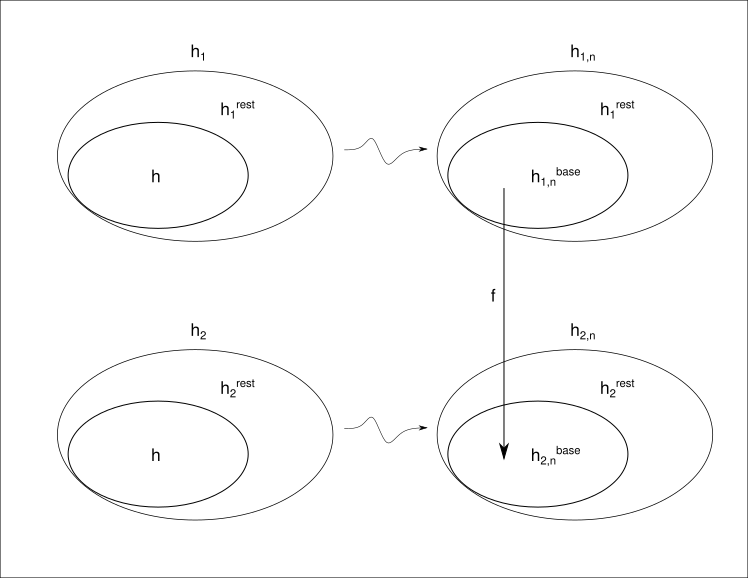
\includegraphics[height=.3\textheight]{ewaluacja_zmienne_wolne.png}
    \end{center}
    \caption{Wizualizacja twierdzenia o zależności ewaluacji od zmiennych wolnych}
    \label{fig:free_vars_eval}
\end{figure}



W praktyce oznacza to, że jedynie fragmenty stert odpowiadające zmiennym wolnym w wyrażeniu
mają znaczenie dla ewaluacji tego wyrażenia.

Dowód twierdzenia będzie przebiegał przez indukcję po długości ewaluacji $\mathit{confs_1}$.
W tym celu jednak musimy sformułować następujący lemat, będący krokiem indukcyjnym w uogólnieniu
powyższego twierdzenia na częściowe ewaluacje.

\begin{lemma}[O zależności redukcji od zmiennych wolnych]{\ } \\
\label{lem:free_red}
Niech $\ctxts_1$ będzie dowolnym stosem wywołań, a $h_1, \hbase_1, \hrest_1$ będą stertami,
takimi że $\hbase_1$ jest spójna , $h_1 = \hbase_1 \oplus \hrest_1$,
a wszystkie lokacje występujące w wyrażeniach na stosie $\ctxts_1$ znajdują się na stercie $\hbase_1$.
Niech teraz $h_{1, n}, \ctxts_{1, n}$ będą takie, że $(h_1, \ctxts_1) \rightarrow (h_{1, n}, \ctxts_{1, n})$.

Weźmy teraz dowolną spójną stertę $\hbase_2$, stos wywołań $\ctxts_2$ oraz izomorfizm $f$,
takie że $f$ jest izomorfizmem między $\hbase_1$ i $\hbase_2$ oraz między $\ctxts_1$ i $\ctxts_2$,
zdefiniowanym tylko na lokacjach znajdujących się w $\hbase_1$.
Jeśli wszystkie lokacje występujące w wyrażeniach na stosie $\ctxts_2$
znajdują się na stercie $\hbase_2$, to dla dowolnych stert $h_2, \hrest_2$, takich że $h_2 = \hbase_2 \oplus \hrest_2$
istnieją sterty $\hbase_{1, n}, \hbase_{2, n}, h_{2, n}$, stos $\ctxts_{2, n}$ oraz izomorfizm $f'$, takie że
\begin{enumerate}
 \item $f'$ rozszerza $f$
 \item $f'$ jest zdefiniowane tylko na lokacjach znajdujących się w $\hbase_{1, n}$
 \item $f'$ jest izomorfizmem między $\hbase_{1,n}$ i $\hbase_{2,n}$ oraz między $\ctxts_{1,n}$ i $\ctxts_{2,n}$
 \item $h_{1, n} = \hbase_{1, n} \oplus \hrest_1$
 \item $h_{2, n} = \hbase_{2, n} \oplus \hrest_2$
 \item wszystkie lokacje występujące w wyrażeniach na stosie $\ctxts_{1, n}$ znajdują się na stercie $\hbase_{1, n}$
 \item wszystkie lokacje występujące w wyrażeniach na stosie $\ctxts_{2, n}$ znajdują się na stercie $\hbase_{2, n}$
 \item $(h_2, \ctxts_2) \rightarrow (h_{2, n}, \ctxts_{2, n})$.
\end{enumerate}
\begin{proof}
Rozpatrzmy wszystkie możliwe postaci izomorficznych stosów $\ctxts_1, \ctxts_2$, takich że istnieje redukcja 
$(h_1, \ctxts_1) \rightarrow (h_{1, n}, \ctxts_{1, n})$.
\begin{itemize}
 \item $\ctxts_1 = \ctxts_1'::\ctxt_1\[ \newin{\mmod}{C}{l_1,\ldots,l_k} \]_\emptyset$, \;\;
 $\ctxts_2 = \ctxts_2'::\ctxt_2\[ \newin{\mmod}{C}{l_1',\ldots,l_k'}\]_\emptyset$ \\ \\
 Redukcja $\ctxts_1$ jest postaci
 $(h_1,  \ctxts_1':: \ctxt_1\[ \newin{\mmod}{C}{l_1,\ldots,l_k}\] _\emptyset) \rightarrow (h_{1, n}, \ctxts_1' :: \ctxt_1\[ l_0\] _\emptyset)$,
gdzie
$ \alloc(h_1, \ctxts_1', C)=(l_0, h),\; \fields(C) = x_1, \dots, x_k,\;
o=\emptyclass{C}\{x_1 \mapsto  l_1,\ldots,x_k~\mapsto~l_k\}, \; h_{1,n} = h\{l_0 \mapsto o\}$.
Nowa sterta $h_{1,n}$ jest zatem po prostu stertą $h_1$ z dodatkowym nowym obiektem $o$ pod nową lokacją $l_0$.
Weźmy zatem $\hbase_{1,n} = \hbase_1\{l_0 \mapsto o\}$.
Spełnia ona warunki 4 i 6, ponieważ jedyną nową lokacją na stosie jest $l_0$, które trafiło właśnie do $\hbase_{1,n}$.

Weźmy teraz $(l_0', h') = \alloc(h_2, \ctxts_2', C),\;
o'=\emptyclass{C}\{x_1 \mapsto  l_1',\ldots,x_k \mapsto  l_k'\}, \; h_{2,n} = h'\{l_0' \mapsto  o'\}$.
Mamy wtedy 
$(h_2, \ctxts_2) \rightarrow (h_{2, n}, \ctxts_2' :: \ctxt_2\[ l_0'\] _\emptyset))$, a zatem biorąc takie $h_{2, n}$
i $\ctxts_{2,n} = \ctxts_2' :: \ctxt_2\[ l_0'\] _\emptyset$ mamy spełnione też warunki 7 i 8.

Jest to jedyny przypadek, w którym na stercie pojawia się nowa lokacja, a zatem należy zmodyfikować
izomorfizm $f$.
Niech więc $\hbase_{2,n} = \hbase_2\{l_0' \mapsto o'\}$ i $f' = f\{l_0 \mapsto l_0'\}$.
Warunki 1 i 5 są w oczywisty sposób spełnione.
Warunek 2 jest spełniony, ponieważ z założenia $f$ było zdefiniowane tylko na lokacjach z $\hbase_1$, a $l_0$ trafiło do $\hbase_{1,n}$.
Wreszcie, warunek 3 jest spełniony, ponieważ z założenia o izomorfizmie $\ctxts_1$ i $\ctxts_2$,
dla $j = 1, \ldots, k$ mamy $f'(l_j) = l_j'$, a z definicji $f'$, $f'(l_0) = l_0'$.

\item $\ctxts_1 = \ctxts_1'::\ctxt_1\[\letin{C}{x}{e_1}{e_2}\]_\emptyset$, \;\;
      $\ctxts_2 = \ctxts_2'::\ctxt_2\[\letin{C}{x}{e_1'}{e_2'}\]_\emptyset$
      
Redukcja $\ctxts_1$ jest postaci
$(h_1, \ctxts_1' :: \ctxt_1\[ \letin{C}{x}{e_1}{e_2}\] _\emptyset) \rightarrow
 (h_1, \ctxts_1' :: \ctxt_1 [\letin{C}{x}{\[ e_1\] _\emptyset}{e_2}])$, a zatem
jedyne co się w niej dzieje to dodanie $e_2$ do kontekstu i zmiana redeksu na $e_1$.

Możemy więc wziąć
$\ctxts_{2,n} = \ctxts_2' :: \ctxt_2 [\letin{C}{x}{\[ e_1'\] _\emptyset}{e_2'}])$,
a sterty i izomorfizm $f$ pozostawić bez zmian.

\item $\ctxts_1 = \ctxts_1'::\ctxt_1[\letin{C}{x}{\[ l\] _\emptyset}{e}]$, \;\;
      $\ctxts_2 = \ctxts_2'::\ctxt_2[\letin{C}{x}{\[ l'\] _\emptyset}{e'}]$
      
Redukcja $\ctxts_1$ jest postaci
$(h_1, \ctxts_1' :: \ctxt_1[\letin{C}{x}{\[ l\] _\emptyset}{e}]) \rightarrow
 (h_1, \ctxts_1' :: \ctxt_1\[ e\{l/x\}\] _\emptyset)$.
Podobnie jak wyżej, możemy pozostawić sterty oraz izomorfizm bez zmian i przyjąć
$\ctxts_{2,n} = (h_2, \ctxts_2' :: \ctxt_2\[ e'\{l'/x\}\] _\emptyset)$.

Wyrażenia $e\{l/x\}$ i $e'\{l'/x\}$ są izomorficzne, ponieważ z założenia $f$ jest izomorfizmem
między $e$ i $e'$ oraz $f(l) = l'$.

\item $\ctxts_1 = \ctxts_1'::\ctxt_1\[\ite{ l_0 == l_1}{e_1}{e_2}\]_\emptyset$, \;\;
      $\ctxts_2 = \ctxts_2'::\ctxt_2\[\ite{ l_0' == l_1'}{e_1'}{e_2'}\]_\emptyset$
      
Redukcja $\ctxts_1$ jest postaci
$(h_1, \ctxts_1'::\ctxt_1\[ \ite{ l_0 == l_1}{e_1}{e_2}\] _\emptyset\!) \rightarrow \!(h_1, \ctxts_1':: \ctxt_1\[ e_i \] _\emptyset)$,
gdzie $i \in \{ 1,2 \}$ w zależności od tego czy $l_0 = l_1$.

Ponieważ $l_0' = f(l_0)$ i $l_1' = f(l_1)$, więc $l_0' = l_1'$ wtedy i tylko wtedy gdy $l_0 = l_1$.
Redukcja $\ctxts_2$ zatem wybierze tę samą gałąź, co redukcja $\ctxts_1$.
Możemy więc wziąć $\ctxts_{2,n} = \ctxts_2'::\ctxt_2\[ e_i' \]_\emptyset$,
a sterty i izomorfizm $f$ pozostawić bez zmian.
      
\item $\ctxts_1 = \ctxts_1'::\ctxt_1\[ l.m(\overline{l})\]_\emptyset$, \;\;
      $\ctxts_2 = \ctxts_2'::\ctxt_2\[ l'.m(\overline{l'})\]_\emptyset$, \;\;
      $l \neq \jnull$
      
Redukcja $\ctxts_1$ jest postaci
$(h_1, \ctxts_1 :: \ctxt_1 \[ l.m(\overline{l})\]_\emptyset) \rightarrow
 (h_1, \ctxts_1 :: \ctxt_1 \[ l.m(\overline{l})\]_\emptyset::\[ e\]_\emptyset)$, gdzie
$e$ jest ciałem metody $m$ z wartościami $\overline{l}$ podstawionymi w miejsce argumentów.

Niech teraz $e'$ będzie ciałem metody $m$ z wartościami $\overline{l'}$
podstawionymi w miejsce argumentów.
Ponieważ listy argumentów $\overline{l}$ i $\overline{l'}$ są izomorficzne, więc wyrażenia
$e$ i $e'$ są izomorficzne.

Możemy więc wziąć
$ \ctxts_{2,n} = \ctxts_2 :: \ctxt_2 \[ l'.m(\overline{l'})\]_\emptyset::\[ e' \]_\emptyset$,
a sterty i izomorfizm pozostawić bez zmian.

\item $\ctxts_1 = \ctxts_1'::\ctxt_1\[ l_1.m(\overline{l})\]_\emptyset :: \[ l_2 \]_\emptyset$, \;\;
      $\ctxts_2 = \ctxts_2'::\ctxt_2\[ l_1'.m(\overline{l'})\]_\emptyset :: \[ l_2' \]_\emptyset$
      
Redukcja $\ctxts_1$ jest postaci
$(h_1, \ctxts_1'::\ctxt_1\[ l_1.m(\overline{l})\]_\emptyset :: \[ l_2 \]_\emptyset) \rightarrow
 (h_1, \ctxts_1'::\ctxt_1\[ l_2\]_\emptyset)$.
Następuje więc jedynie zdjęcie wywołania metody ze stosu wywołań.
Możemy zatem wziąć
$\ctxts_{2,n} = \ctxts_2'::\ctxt_2\[ l_2'\]_\emptyset$, a sterty i izomorfizm pozostawić bez zmian.

\item $\ctxts_1 = \ctxts_1'::\ctxt_1\[ l_1.x = l\]_\emptyset$, \;\;
      $\ctxts_2 = \ctxts_2'::\ctxt_2\[ l_1'.x = l'\]_\emptyset$, \;\;
      $l_1 \neq \jnull$
      
Redukcja $\ctxts_1$ jest postaci
$(h_1,  \ctxts_1'::\ctxt_1\[ l_1.x = l\]_\emptyset) \rightarrow
 (h_{1, n},\; \ctxts_1'::\ctxt_1\[ l\]_\emptyset)$, gdzie
$o = h_1(l_1)\{x \mapsto  l\}$, $h_{1,n} = h_1\{l_1 \mapsto o\}$

Ponieważ izomorfizm jest różnowartościowy i zachowuje $\jnull$, więc również $l_1' \neq \jnull$.
Weźmy zatem
$o' = h_2(l_1')\{x \mapsto  l'\}$, $h_{2,n} = h_2\{l_1' \mapsto o'\}$ i
$h_{2,n}^{base} = h_2^{base}\{l_1' \mapsto o'\}$.

Możemy teraz wziąć $\ctxts_{2,n} = \ctxts_2'::\ctxt_2\[ l'\]_\emptyset$ i
pozostawić izomorfizm $f$ bez zmian.

\item $\ctxts_1 = \ctxts_1'::\ctxt_1\[ l_1.x\]_\emptyset$, \;\;
      $\ctxts_2 = \ctxts_2'::\ctxt_2\[ l_1'.x\]_\emptyset$, \;\;
      $l \neq \jnull$
      
Redukcja $\ctxts_1$ jest postaci
$(h_1, \ctxts_1'::\ctxt_1\[ l_1.x\]_\emptyset) \rightarrow
 (h_1, \ctxts_1'::\ctxt\[ l_2\]_\emptyset)$,
gdzie $l_2=h_1(l_1)(x)$.

Ponieważ sterty $h_1$ i $h_2$ są izomorficzne, więc na stercie $h_2$ istnieje obiekt pod lokacją
$l_1'$ zawierający pole $x$ i, co więcej, jeśli $l_2' = h_2(l_1')(x)$, to $f(l_2) = l_2'$.

Zatem możemy wziąć $\ctxts_{2, n} = \ctxts_2'::\ctxt\[ l_2'\]_\emptyset$, a sterty
i izomorfizm pozostawić bez zmian.

\item $\ctxts_1 = \ctxts_1'::\ctxt_1\[ \throwin{l}\]_\emptyset$, \;\;
      $\ctxts_2 = \ctxts_2'::\ctxt_2\[ \throwin{l'}\]_\emptyset$, \;\;
      $l \neq \jnull$

Redukcja $\ctxts_1$ jest postaci
 $(h_1, \ctxts_1'::\ctxt_1\[ \throwin{l}\]_\emptyset) \rightarrow
  (h_1, \ctxts_1'::\ctxt_1\[ l\]_{D})$, gdzie $\classof(h_1, l) = D$, zatem jedynym efektem
jest zmiana trybu wykonania na wyjątkowy z wartością wyjątku $l$ i typem $D$.
Możemy więc po prostu wziąć $\ctxts_{2, n} = \ctxts_2'::\ctxt_2\[ l'\]_{D}$,
a sterty i izomorfizm pozostawić bez zmian.

\item $\ctxts_1 = \ctxts_1'::\ctxt_1\[ \tcatch{e_1}{\mmod\; C}{x}{e_2}\]_\emptyset$, \;\;
      $\ctxts_2 = \ctxts_2'::\ctxt_2\[ \tcatch{e_1'}{\mmod\; C}{x}{e_2'}\]_\emptyset$

Redukcja $\ctxts_1$ jest postaci
$(h_1, \ctxts_1'::\ctxt_1\[ \tcatch{e_1}{\mmod\; C}{x}{e_2}\]_\emptyset) \rightarrow
 (h_1, \ctxts_1'::\ctxt_1[\tcatch{\[ e_1\] _\emptyset}{\mmod\; C}{x}{e_2}])$,
a zatem przebiega podobnie, jak analogiczna redukcja dla $\jlet$ -- do kontekstu dodawane jest
wyrażenie $e_2$, a redeks zostaje zmieniony na $e_1$. Podobnie jak dla $\jlet$, możemy wziąć
$\ctxts_{2, n} = \ctxts_2'::\ctxt_2[\tcatch{\[ e_1'\] _\emptyset}{\mmod\; C}{x}{e_2'}])$,
a sterty i izomorfizm pozostawić bez zmian.

\item $\ctxts_1 = \ctxts_1'::\ctxt_1[\tcatch{\[ l\] _\emptyset}{\mmod\; C}{x}{e_2}]$, \;\;
      $\ctxts_2 = \ctxts_2'::\ctxt_2[\tcatch{\[ l'\] _\emptyset}{\mmod\; C}{x}{e_2'}]$

Przy normalnym wykonaniu wyrażenia wewnątrz blocku $\jtry$, jest on po prostu usuwany z kontekstu.
Redukcja $\ctxts_1$ jest wtedy postaci
$(h_1, \ctxts_1'::\ctxt_1[\tcatch{\[ l\] _\emptyset}{\mmod\; C}{x}{e_2}]) \rightarrow
 (h_1, \ctxts_1'::\ctxt_1\[ l\]_\emptyset)$.
 
Wystarczy zatem wziąć $\ctxts_{2,n} = \ctxts_2'::\ctxt_2\[ l'\]_\emptyset$,
a sterty i izomorfizm pozostawić bez zmian.

\item $\ctxts_1 = \ctxts_1'::\ctxt_1[\tcatch{\[ l\] _{C'}}{\mmod\; C}{x}{e_2}]$, \;\;
      $\ctxts_2 = \ctxts_2'::\ctxt_2[\tcatch{\[ l'\] _{C'}}{\mmod\; C}{x}{e_2'}]$, \;\;
      gdzie $C' \leq:  C $
      
Redukcja w tym przypadku oznacza złapanie rzuconego wcześniej wyjątku i obsłużenie go przez $e_2$.
Jest ona postaci
$(h_1, \ctxts_1'::\ctxt_1[\tcatch{\[ l\] _{C'}}{\mmod\; C}{x}{e_2}]) \rightarrow
 (h_1, \ctxts_1'::\ctxt_1\[ e\]_\emptyset)$, gdzie $e = e_2\{l/x\}$.

Niech $e' = e_2'\{l' / x\}$. Wtedy wystarczy wziąć
$\ctxts_{2,n} = \ctxts_2'::\ctxt_2\[ e'\]_\emptyset$, a sterty i izomorfizm pozostawić bez zmian.

\item $\ctxts_1 = \ctxts_1'::\ctxt_1[\tcatch{\[ l\] _{C'}}{\mmod\; C}{x}{e_2}]$, \;\;
      $\ctxts_2 = \ctxts_2'::\ctxt_2[\tcatch{\[ l'\] _{C'}}{\mmod\; C}{x}{e_2'}]$, \;\;
      gdzie $C'\not=\emptyset, C' \not\!\leq:  C $  

W przypadku niezłapanie wyjątku, kontekst $\jtry$ jest usuwany, a wyjątek przekazywany dalej.
Redukcja jest postaci
$(h_1, \ctxts_1'::\ctxt_1[\tcatch{\[ l\] _{C'}}{\mmod\; C}{x}{e_2}]) \rightarrow
 (h_1, \ctxts_1'::\ctxt_1\[ l\] _{C'})$.
Bierzemy zatem $\ctxts_{2,n} = \ctxts_2'::\ctxt_2\[ l'\] _{C'}$,
a sterty i izomorfizm pozostawiamy bez zmian.
 
\item $\ctxts_1 = \ctxts_1'::\ctxt_1[\letin{C}{x}{\[ l\] _{C'}}{e}]$, \;\;
      $\ctxts_2 = \ctxts_2'::\ctxt_2[\letin{C}{x}{\[ l'\] _{C'}}{e'}]$, \;\;
      $C' \neq \emptyset$
      
Przypadek wyjątku w czasie ewaluacji wyrażenia wewnętrzego $\jlet$ jest analogiczny jak
poprzedni. Możemy wziąć $\ctxts_{2,n} = \ctxts_2'::\ctxt_2\[ l'\] _{C'}$,
a sterty i izomorfizm zostawić bez zmian.
      
\item $\ctxts_1 = \ctxts_1'::\ctxt_1\[ l_1.m(\overline{l})\]_\emptyset::\[l_2\]_C$, \;\;
      $\ctxts_2 = \ctxts_2'::\ctxt_2\[ l_1'.m(\overline{l'})\]_\emptyset::\[l_2'\]_C$, \;\;
      $C\not=\emptyset$  
      
Podobnie w przypadku wyjątku podczas wykonywania metody. Wywołanie jest zdejmowane ze stosu,
a wyjątek przekazywany wyżej. Redukcja jest postaci
$(h_1, \ctxts_1'::\ctxt_1\[ l_1.m(\overline{l})\]_\emptyset::\[l_2\]_C) \rightarrow
 (h_1, \ctxts_1'::\[l_2\]_C)$.
 
Bierzemy $\ctxts_{2,n} = (h_1, \ctxts_2'::\[l_2'\]_C)$, a sterty i izomorfizm pozostawiamy bez zmian.

 
\item Redukcja $\ctxts_1$ powoduje odwołanie do lokacji $\jnull$

Jest tak, gdy $\ctxts_1 = \ctxts_1'::\ctxt_1\[e\]_\emptyset$, gdzie
$e$ jest postaci  $\jnull.x$, $\jnull.x = l$, $\jnull.m( \overline{l})$ lub
$\throwin{\jnull}$.
 
Redukcja $\ctxts_1$ jest wtedy postaci
$(h_1, \ctxts_1':: \ctxt_1 \[ e \]_\emptyset) \rightarrow
 (h_1, \ctxts_1':: \ctxt_1 \[ \npe\]_\npetype)$.
 
Wówczas $\ctxts_2 = \ctxts_2'::\ctxt_2 \[ e' \]_\emptyset$, gdzie $e'$ jest izomorficzne z $e$,
a ponieważ izomorfizm zachowuje $\jnull$ więc redukcja $e'$ również powoduje
odwołanie do $\jnull$.

Ponieważ izomorfizm zachowuje także $\npe$, możemy wziąć
$\ctxts_{2,n} = \ctxts_2'::\ctxt_2 \[ \npe \]_\npetype$,
a sterty i izomorfizm pozostawić bez zmian.
\end{itemize}
\end{proof}
\end{lemma}

Korzystając z tego lematu w kroku indukcyjnym udowodnimy teraz następujący lemat,
mówiący o ewaluacjach dowolnej długości.

\begin{lemma}[O zależności częsciowej ewaluacji od zmiennych wolnych]{\ } \\
\label{lem:free_part_eval}
Niech $\ctxts_1$ będzie dowolnym stosem wywołań, a $h_1, \hbase_1, \hrest_1$ będą stertami,
takimi że $\hbase_1$ jest spójna , $h_1 = \hbase_1 \oplus \hrest_1$,
a wszystkie lokacje występujące w wyrażeniach na stosie $\ctxts_1$ znajdują się na stercie $\hbase_1$.
Niech teraz $h_{1, n}, \ctxts_{1, n}, \mathit{confs}_1$ będą takie,
że $(h_1, \ctxts_1) \eval{confs_1} (h_{1, n}, \ctxts_{1, n})$.

Weźmy teraz dowolną spójną stertę $\hbase_2$, stos wywołań $\ctxts_2$ oraz izomorfizm $f$,
takie że $f$ jest izomorfizmem między $\hbase_1$ i $\hbase_2$ oraz między $\ctxts_1$ i $\ctxts_2$,
zdefiniowanym tylko na lokacjach znajdujących się w $\hbase_1$.
Jeśli wszystkie lokacje występujące w wyrażeniach na stosie $\ctxts_2$
znajdują się na stercie $\hbase_2$, to dla dowolnych stert $h_2, \hrest_2$, takich że $h_2 = \hbase_2 \oplus \hrest_2$
istnieją sterty $\hbase_{1, n}, \hbase_{2, n}, h_{2, n}$, stos $\ctxts_{2, n}$, izomorfizm $f'$
oraz ciąg konfiguracji $\mathit{confs}_2$, takie że
\begin{enumerate}
 \item $f'$ rozszerza $f$
 \item $f'$ jest zdefiniowane tylko na lokacjach znajdujących się w $\hbase_{1, n}$
 \item $f'$ jest izomorfizmem między $\hbase_{1,n}$ i $\hbase_{2,n}$ oraz między $\ctxts_{1,n}$ i $\ctxts_{2,n}$
 \item $h_{1, n} = \hbase_{1, n} \oplus \hrest_1$
 \item $h_{2, n} = \hbase_{2, n} \oplus \hrest_2$
 \item wszystkie lokacje występujące w wyrażeniach na stosie $\ctxts_{1, n}$ znajdują się na stercie $\hbase_{1, n}$
 \item wszystkie lokacje występujące w wyrażeniach na stosie $\ctxts_{2, n}$ znajdują się na stercie $\hbase_{2, n}$
 \item $(h_2, \ctxts_2) \eval{confs_2} (h_{2, n}, \ctxts_{2, n})$.
\end{enumerate}
\begin{proof}
Przez indukcję po długości ciągu konfiguracji $\mathit{confs}_1$.
\begin{itemize}
 \item Jeśli $\mathit{confs}_1 = [\ ]$ jest pustym ciągiem, to znaczy że $h_{1,n} = h_1$ oraz
 $\ctxts_{1,n} = \ctxts_1$.
 Możemy wtedy wziąć $h_{1,n}^{base} = h_1^{base}$, $h_{2,n}^{base} = h_2^{base}$,
 $h_{2,n} = h_2$, $\ctxts_{2,n} = \ctxts_2$, $f' = f$ oraz $\mathit{confs}_2 = [\ ]$.
 \item Jeśli $\mathit{confs}_1 = \mathit{confs'}_1 :: (h_{1,n-1}, \ctxts_{1,n-1})$, to
 Z założenia indukcyjnego będziemy mieli
 sterty $\hbase_{1, n-1}, \hbase_{2, n-1}, h_{2, n-1}$, stos $\ctxts_{2, n-1}$, izomorfizm $f'$
 oraz ciąg konfiguracji $\mathit{confs'}_2$, takie że spełnione są warunki z treści zadania,
 w szczególności $(h_2, \ctxts_2) \eval{confs'_2} (h_{2,n-1}, \ctxts_{2, n-1})$.
 Z lematu \ref{lem:free_red} dostaniemy 
 sterty $\hbase_{1, n}, \hbase_{2, n}, h_{2, n}$, stos $\ctxts_{2, n}$ oraz izomorfizm $f''$, takie że
 spełnione są warunki 1-7 oraz
 $(h_{2,n-1}, \ctxts_{2,n-1}) \rightarrow (h_{2, n}, \ctxts_{2, n})$.
 Składając tę redukcję z ewaluacją z założenia indukcyjnego dostaniemy, że w istocie
 $(h_2, \ctxts_2) \eval{confs_2} (h_{2, n}, \ctxts_{2, n})$.
\end{itemize}
\end{proof}
\end{lemma}

Możemy wreszcie udowodnić twierdzenie \ref{th:free_eval}
\begin{proof} (twierdzenia o zależności ewaluacji od zmiennych wolnych)
    Niech $h$, $env$, $E$, $h_1$, $h_2$, $\hrest_1$, $\hrest_2$, $\mathit{confs_1}, h_{1,n}, A, l_1$
    będą jak w treści twierdzenia.
    Pokażę, że istnieją istnieją  $\hbase_{1, n}, \hbase_{2, n}, \mathit{confs}_2, h_{2, n}, l_2, f$,
    spełniające warunki z treści.
    
    W tym celu zastosujemy lemat \ref{lem:free_part_eval} dla
    $\hbase_1 = \hbase_2 = h$, ewaluacji
    $(h_1, \[ E[/env] \]_\emptyset) \eval{confs_1} (h_{1,n}, \[ l_1 \]_A)$ i
    $\ctxts_2 = \[ E[/env] \]_\emptyset$.
    Żeby jednak móc go zastosować, musimy pokazać że wszystkie lokacje z wyrażenia $E[/env]$
    występują na stercie $h$. Wynika to jednak wprost z założeń, że w wyrażeniu $E$ nie ma
    konkretnych lokacji, a wszystkie zmienne wolne mapowane są przez $env$ na lokacje z $h$.
    Stąd, po podstawieniu za zmienne wolne lokacji z $env$, założenie jest spełnione.
    
    Ostatnim problemem jest wybranie odpowiedniego początkowego $f$.
    Wystarczy jednak, żeby $f$ była identycznością na $\jnull$, $\npe$ i lokacjach występująych
    w $h$ lub $E[/env]$. Ponieważ $h$ jest spójna, więc tak zdefiniowana $f$ jest w oczywisty sposób
    automorfizmem na $h$ oraz na $E[/env]$.
\end{proof}

\chapter{Poprawność}
Głównym twierdzeniem, dowodzonym w ramach niniejszej pracy, jest poprawność prezentowanej logiki.
Mówi ono, że jeśli możemy udowodnić pewne wynikanie $\Gamma | P \vdash Q$,
to każda sterta spełniająca $P$ będzie również spełniała $Q$.
Dla ścisłego sformułowania tego twierdzenia potrzebujemy jednak kilku dodatkowych założeń o stertach
i programach, o których chcemy wnioskować.

\section{Konieczne założenia}
Będziemy rozważać jedynie spójne sterty. Ponieważ język Jafun jest silnie typowany, więc potrzebne
jest także założenie o odpowiednim otypowaniu obiektów na stercie.
Powiemy więc, że środowisko $\mathit{env}$ zgadza się ze środowiskiem typów $\Gamma$ na stercie $h$,
jeśli mają te same dziedziny i typ każdej zmiennej w $\Gamma$ zgadza się z jej typem na stercie $h$.
To znaczy, dla każdego $x$, jesli $\Gamma \vdash x : C$, to obiekt $h(\mathit{env}(x))$ jest typu $C$.

W twierdzeniu o poprawności będziemy wymagać, żeby rozważane środowisko było zgodne z $\Gamma$
na stercie, o której będziemy wnioskować. W połączeniu z założeniem o tym, że wszystkie zmienne wolne
pojawiąjące się w osądach muszą być w $\Gamma$, zapewni to, że wszystkie zmienne wolne są mapowane
przez środowisko na pewną lokację istniejącą na stercie i, co więcej, obiekt znajduący się pod tą
lokacją jest odpowiedniego typu.

Wreszcie, należy poczynić odpowiednie założenia o niezmiennikach.
Lista niezmienników została wprowadzona w rozdziale \ref{chap:rules} jako lista elementów postaci
$(C, m, \hoare{P}{\cdot}{A}{w}{Q})$.
Każdy taki niezmiennik oznaczał założenie o własności ewaluacji metody $m$ na obiektach klasy
$C$ i jej pochodnych.
Żeby jednak takie założenie było poprawne, należy zadbać o to, żeby każdy taki niezmiennik dał
się wyprowadzić korzystając z reguł dowodzenia i niezmienników będących wcześniej na liście.
Pozwoli to udowodnić poprawność każdego z nich przez prostą indukcję po długości listy niezmienników.

Zdefiniujmy więc \textit{udowodnioną listę niezminników} indukcyjnie, w następujący sposób.
Powiemy, że pusta lista niezmienników jest udowodniona.
Niepusta lista niezmienników $\mathtt{invariants}::(C, m, \hoare{P}{\cdot}{A}{w}{Q})$ dla
programu $\overline{\mathbf{C}}$ jest
udowodniona wtedy i tylko wtedy, gdy udowodniona jest lista $\mathtt{invariants}$ oraz osąd
$\overline{\mathbf{C}}, \mathtt{invariants}, \Gamma | \mathtt{True} \vdash \hoare{P}{E}{A}{w}{Q}$
jest wyprowadzalny dla każdego $E$ będącego ciałem metody $m$ w klasie $C$ lub jej pochodnej i
dla $\Gamma$ będącej środowiskiem typów przypisującym nazwom argumentów metody
$m$ ich typy, a wartości $\jthis$ typ $C$.

Zauważmy, że warunek dodania niezmiennika do listy jest bardzo silny -- należy udowodnić jego
prawdziwość nie tylko dla metody w interesującej nas klasie, ale również dla każdego jej przeciążonego
odpowiednika w klasach pochodnych. Z jednej strony ogranicza to zakres wnioskowania o metodach,
ale z drugiej wymusza pewną dyscyplinę podczas przeciążania metod.
Definiując metodę z intencją jej przeciążenia należy bowiem zastanowić się, jakie własności
powinna ona spełniać we wszystkich klasach pochodnych.
Dzięki temu można zapewnić, że metoda ta we wszystkich klasach dziedziczących zachowuje się
w podobny, dobrze określony sposób.

\section{Twierdzenie o poprawności}

Możemy teraz ściśle sformułować twierdzenie o poprawności.
\begin{theorem}[O poprawności logiki separacji dla języka Jafun]{\ } \\
  Niech $\overline{\mathbf{C}}$ będzie programem języka Jafun i niech $\mathtt{invariants}$
  będzie udowodnioną listą niezmienników.
  Niech $P, Q$ będą dowolnymi termami logiki separacji, takimi że $\Gamma | P \vdash Q$.
  Wtedy dla każdej spójnej sterty $h$ i środowiska $\mathit{env}$, takich że $\mathit{env}$ zgadza się z $\Gamma$
  na stercie $h$ mamy $\[ P \]_{h, env} = \[ Q \]_{h, env}$.
  \qed
\end{theorem}

Dowód tego twierdzenia przebiega w pierdzej kolejności przez indukcję po
długości listy niezmienników, a następnie przez indukcję po budowie drzewa dowodu
dla $\Gamma | P \vdash Q$.
Najpierw należy pokazać, poprawność przypadków bazowych, czyli udowodnić tezę twierdzenia dla
wszystkich reguł niezawierających osądów w przesłankach.
Następnie należy pokazać, że wszystkie pozostałe reguły zachowują poprawność.
W tym celu będziemy zakładać, że wszystkie osądy z przesłanek są poprawne,
a następnie korzystając z tych założeń będziemy dowodzić poprawność osądu będącego wnioskiem reguły.
Takie założenie jest możliwe dzięki temu, że drzewa dowodów przesłanek są właściwymi poddrzewami
dowodu dla wniosku, a zatem założenie o poprawności przesłanek jest założeniem indukcyjnym.

Dowód tego twierdzenia w systemie Coq znajduje się w pliku \texttt{JaIrisSoundeness.v}
jako dowód twierdzenia \texttt{JFIOuterSoundness}.

\section{Poprawność reguł dla tradycyjnych operatorów logicznych}
Dowody poprawności reguł przedstawionych na rysunku \ref{fig:logical_rules} są do siebie
bardzo podobne i,~oprócz kilku szczegółów techniczych, mało interesujące, jako że wprost
wynikają z własności operatorów logicznych.
Na przykład, poprawność reguły \textsc{Asm} jest oczywista -- każda sterta spełniająca $P$ spełnia $P$.

Dowód poprawności innych reguł jednak wymaga doprecyzowania.
Poprawność reguły \textsc{Trans} wymaga pokazania, że zmienna $v$ istnieje w środowisku $\mathit{env}$.
Jest to prawdą, ponieważ z faktu, że $v$ jest zmienną wolną w osądzie wynika, że $v$ ma przypisany
typ w środowisku typów $\Gamma$.
Istnienie $v$ w środowisku $\mathit{env}$ wynika więc z założenia o zgodności $\mathit{env}$ i~$\Gamma$ 

Kolejną regułą, której poprawność jest nieoczywista, jest reguła $\exists \mathrm{I}$,
wprowadzająca kwantyfikator $\exists$.
Należy tu pokazać, że, zakładając poprawność przesłanki, każda sterta spełniająca
$Q$ spełnia też $\exists x : C . P$.
Kluczową rolę gra tutaj wartość $v$, którą podstawiamy za zmienną $x$.
Należy rozpatrzeć przypadki, w których $v$ jest równa $\jnull$, $\jthis$ lub jest zmienną.
Następnie możemy dodać do środowiska mapowanie $x$ na odpowiednio $\jnull$, $env(\jthis)$ lub $env(v)$.
Powstałe środowisko jest wtedy zgodne ze środowiskiem $(\Gamma, x : C)$ na stercie $h$,
a zatem można po prostu zastosować założenie indukcyjne.

Wreszcie, najbardziej najbardziej skomplikowanym przypadkiem, spośród reguł dla klasycznych operatorów,
jest poprawność reguły $\exists\mathrm{E}$, eliminującej kwantyfikator $\exists$.

Kluczowym krokiem w dowodzie poprawności $\exists\mathrm{E}$ jest zauważenie, że dodanie świeżej,
nie będącej zmienną wolną w termie,
zmiennej do środowiska nie zmienia spełnialności tego termu przez stertę.
To znaczy jeśli $x \not\in FV(P)$, to $\[ P \]_{h, env} = \[ P \]_{h, env[x \mapsto l]}$.
Formalny dowód tego faktu wymaga indukcji po budowie termu $P$, ale intuicyjnie jest to prawda,
ponieważ skoro $x$ nie jest wolne w $P$, więc $P$ nie ma możliwości odwoływania się do niego,
a zatem podczas obliczania semantyki $P$ w środowisku $\mathit{env}$ nigdy nie odwołamy się
do lokacji $env(x)$. Nie ma zatem znaczenia, czy $x$ występuje w środowisku $\mathit{env}$ i,
jeśli tak, to jaka jest wartość $env(x)$.

Kiedy udowodnimy ten fakt, reszta dowodu przebiega już w prosty sposób:
mamy stertę $h$ oraz środowisko $env$ zgadzające się na $h$ z $\Gamma$, takie że
$h$ spełnia term $R$ w środowisku $env$. Skoro tak, to z założenia indukcyjnego dla
pierwszej przesłanki mamy, że $h$ spełnia też w tym środowisku term $\exists x : C . P$, a zatem
istnieje taka lokacja $l$, że $h(l)$ jest typu $C$ i $h$ spełnia $P$ w środowisku $env[x \mapsto l]$.

Możemy więc teraz zastosować założenie indukcyjne dla drugiej przesłanki.
Jak zauważyliśmy przed chwilą, $env[x \mapsto l]$ zgadza się z $(\Gamma, x : C)$ na stercie $h$ oraz
$h$ spełnia $P$ w tym środowisku. Pozostaje pokazać, że $h$ spełnia $R$ w tym środowisku.
W tym momencie korzystamy z obserwacji o zachowaniu spełniania przy dodaniu świeżej zmiennej.
Wiemy, że $h$ spełnia $R$ w środowisku $env$, oraz że $x$ jest świeże w $R$
(bo $x$ nie jest w $\Gamma$, a wszystkie zmienne wolne z $R$ są).
$h$ spełnia więc też $R$ w środowisku $env[x \mapsto l]$, a zatem z założenia indukcyjnego dla
drugiej przesłanki, $h$ spełnia $Q$ w środowisku $env[x \mapsto l]$.

Możemy teraz ponownie skorzystać z faktu o świeżych zmiennych, bo, podobnie jak w $R$,
$x$ jest świeże w $Q$. Ostatecznie dostajemy więc, że $h$ spełnia $Q$ w środowisku $env$, a zatem
reguła $\exists\mathrm{E}$ jest poprawna.

\section{Poprawność reguł dla operatorów separacji}
Poprawność reguł \textsc{Sep-assoc} i \textsc{Sep-sym} wynika w prosty sposób z własności sterty,
takich jak przemienność i łączność operatora $\oplus$ oraz faktu że suma spójnych stert jest spójna.
Poprawność pozostałych reguł jest nieco bardziej skomplikowanym zagadnieniem.

\subsection{Reguły eliminacji i wprowadzania operatorów separacji}
Dowód poprawności eliminacji i wprowadzania operatorów separacji nie jest skompliowany,
ale kryje się w nim kilka subtelności związanych z manipulowaniem środowiskami, tak
żeby było możliwe skorzystanie z nich używając założeń indukcyjnych.
Pokażę je na przykładzie reguły $*\mathrm{I}$, ale podobne rozumowanie jest też stosowane w
pozostałych regułach.

Aby pokazać poprawność tej reguły, bierzemy dowolne spójne $h$ spełniające $P_1 * P_2$ i środowisko
$env$ zgadzające się z $(\Gamma_1, \Gamma_2)$ na $h$.
Ponieważ $h$ spełnia $P_1 * P_2$, więc istnieje podział $h$ na rozłączne sterty $h_1$ i $h_2$,
spełniające odpowiednio $P_1$ i $P_2$. Chcemy teraz skorzystać z założeń indukcyjnych, żeby
otrzymać, że spełniają one też odpowiednio $Q_1$ i $Q_2$, co zakończy dowód.

Nie możemy jednak zrobić tego używając środowiska $env$, bo nie musi ono zgadzać się z $\Gamma_1$
ani $\Gamma_2$ -- jest na to zbyt duże. O ile oba ze środowisk typów są niepuste, to $env$ zawiera
zarówno zmienne niebędące w $\Gamma_1$, jak i zmienne niebędące w $\Gamma_2$.
Należy więc ostrożenie wziąc podzbiór środowiska $env$, zgodny z $\Gamma_1$ na $h_1$ i drugi,
zgodny z $\Gamma_2$ na $h_2$ w taki sposób, żeby zachować spełnianie termów przez sterty
$h_1$ i $h_2$ w tych okrojonych środowiskach.

Aby to osiągnąć, wystarczy wziąć $env_1$ i $env_2$ będące obcięciami środowiska $env$ odpowiednio do
zmiennych znajdujących się w $\Gamma_1$ i $\Gamma_2$.
Wtedy oczywiście $env_1$ zgadza się z $\Gamma_1$ na $h_1$ i analogicznie dla $env_2$.
Pozostaje więc pokazać, że $h_1$ spełnia $P_1$ w środowisku $env_1$.
W tym celu możemy znów skorzystać z faktu, że dodawanie świeżych zmiennych do środowiska nie
wpływa na spełnianie termu przez stertę. Ponieważ wszystkie zmienne wolne w $P_1$ znajdują
się w $\Gamma_1$, więc znajdują się też w $env_1$. Możemy więc otrzymać $env$ przez dodawanie
do $env_1$ kolejnych zmiennych, z których każda jest świeża w $P_1$, a zatem dodanie żadnej z nich
nie zmienia spełniania $P_1$ przez $h_1$. Stąd mamy więc
$\[ P_1 \]_{h_1, env} = \[ P_1 \]_{h_1, env_1}$ i podobnie
$\[ Q_1 \]_{h_1, env} = \[ Q_1 \]_{h_1, env_1}$.

Korzystając więc z powyższych równości i z założenia indukcyjnego, dostajemy że $h_1$ spełnia $Q_1$
w środowisku $env$. Przeprowadzenie analogicznego rozumowania dla $h_2$ kończy dowód.

\subsection{Reguła osłabiania}
Reguła osłabiania \textsc{*-Weak} jest jedną z dwóch reguł, obok reguły \textsc{Ht-frame},
dzięki którym operatory separacji są tak przydatne.
Sprawia ona, że logika separacji jest afiniczna, to znaczy że jeśli sterta spełnia pewien term,
to każda jej spójna nadsterta też go spełnia.

Istotnie, skoro mamy $P_1 * P_2 \vdash P_1$ dla dowolnych $P_1, P_2$,
to po przyjęciu $P_2 = \texttt{True}$ możemy w pewnym sensie zapomnieć o niepasującej nam części
sterty. Jeśli mamy więc stertę $h_1$ spełniającą term $P_1$, to dla dowolnej sterty $h_2$ mamy
$h_1 \oplus h_2$ spełnia $P_1 * \mathtt{True}$, a zatem, korzystając z reguły osłabiania, także
$h_1 \oplus h_2$ spełnia $P_1$.

Jest to niewątpliwie silna własność logiki, jednak zachować jej poprawność przy zadanej semantyce
języka, niezbędne były pewne kompromisy. Przede wszystkim, logika ta nie zawiera kwantyfikatora
ogólnego $\forall$. Przy naszej definicji sterty kwantyfikator ten zaburzyłby poprawność reguły
osłabiania. Bez dodatkowych założeń nie ma bowiem gwarancji, że $h_1 \oplus h_2$ spełnia
$\forall x . P$, nawet jeśli samo $h_1$ spełnia $\forall x . P$. Podczas rozszerzania sterty moglibyśmy
dodać nowe lokacje, niespełniające $P$, i w ten sposób zepsuć poprawność tej reguły.

Jednocześnie, nięzbędne jest też zadbanie, żeby nie było możliwe symulowanie kwantyfikatora ogólnego
przy pomocy innych kontrukcji logiki. Możliwe byłoby to na przykład przez zastąpienie
termu $\forall x : C . P$ przez $\neg \exists x : C . \neg P$.
Z tego powodu kwantyfikator $\exists$ został w logice ograniczony do termów najwyższego poziomy, tak
że niemożliwe staje się jego zanegowanie.

Te dwa ograniczenia wystarczają do zapewnienia poprawności reguły osłabiania przy zachowaniu
semantyki języka bez zmian.

{\ }

Wciąż jednak, pomimo tych ograniczeń, dowód poprawności reguły osłabiania nie jest trywialny.
Wynika ona wprost z pomocniczego twierdzenia, mówiącego że jeśli pewne środowisko mapuje
wszystkie zmienne wolne termu na lokacje na pewnej stercie, to możemy dowolnie rozszerzać zarówno
środowisko jak i stertę bez zmiany semantyki tego termu, to znaczy jeśli
$h_1 \subseteq h$, $env_1 \subseteq env$ i wszystkie zmienne wolne z termu $P$
mapowane są przez $env_1$ na lokacje w $h_1$, to $\[ P \]_{h_1, env_1} = \[ P \]_{h, env}$.

Twierdzenie to, mimo że wygląda podobnie to przytaczanego wcześniej faktu o rozszerzaniu środowiska
o świeże zmienne, jest od niego istotnie trudniejsze do udowodnienia, ponieważ tutaj chcemy
zagwarantować także możliwość rozszerzania sterty.
Powoduje to utrudnienia w dowodzie dla przypadku trójki Hoare'a. W pozostałych przypadkach
dowód nadal nie jest trudny. Dzięki temu, że operator $*$ może występować jedynie w
wyrażeniach wewnętrznych, nie musimy przejmować się kwantyfikatorem $\exists$.

W przypadku trójek Hoare'a jednak musimy skorzystać z udowodnionego wcześniej twierdzenia
\ref{th:free_eval} (O zależności ewaluacji od zmiennych wolnych).
Zapewnia nam ono, że dla dowolnej ewaluacji na stercie $h_1$ będziemy mieli odpowiednią
ewaluację na stercie $h$ i, co więcej, otrzymane na końcu sterty będą izomorficzne.
Pozostaje więc pokazać, że dla semantyka termu dla izomorficznych stert jest taka sama.
Jest to prawda tylko przy założeniu, że środowiska, w których rozpatrujemy semantykę,
również są izomorficzne, przynajmniej na zmiennych wolnych w tym termie. Na szczęście jednak
twierdzenie \ref{th:free_eval} zapewnia nam, że otrzymany izomorfizm jest identycznością na
lokacjach przypisanych w środowisku, a zatem wyjściowe środowiska $env$ i $env_1$
spełniają to założenie.


\section{Poprawność reguł dla trójek Hoare'a}
Najliczniejszą grupę reguł wnioskowania stanowią, przedstawione na rysunkach
\ref{fig:hoare_rules} i \ref{fig:hoare_rules2}, reguły dla trójek Hoare'a.
Większość z nich jest bardzo prosta, a ich poprawność wynika wprost z semantyki języka.
Do takich należą \textsc{Ht-new-null}, gwarantująca że alokacja obiektu zawsze się powiedzie i zwróci
niepustą lokację, czy \textsc{Ht-null-get}, mówiąca że próba odczytu pola obiektu pod lokacją
$\jnull$ zakończy się rzuceniem wyjątku $\npe$.

Z drugiej strony, dowody poprawności niektórych z nich są skomplikowane lub zawierają
subtelne niuanse. O takich przykładach opowiem poniżej.

Jednym z motywów powtarzających się w wielu regułach dla trójek Hoare'a
jest założenie o trwałości niektórych termów.
Zazwyczaj oznacza to, że w dowodzie poprawności potrzebujemy założenia o spełnianiu takiego
termu przez pewną stertę, przy założeniu, że spełnia go inna sterta.
Ponieważ termy trwałe nie opisują w żaden sposób własności sterty, więc dowolne dwie sterty
są równoważne, jeśli chodzi o spełnianie danego trwałego termu.

\section{Reguły strukturalne}
Dzięki regule \textsc{Ht-frame} możemy w pełni docenić operator separacji $*$.
Upraszcza ona dowodzenie faktów o trójkach Hoare'a na złożonych stertach,
sprawiając że możliwe jest dowodzenie własności ograniczając się tylko do istotnych
dla nich fragmentów sterty, a następnie rozszerzanie tych fragmentów to
interesującej nas całości. Dzięki takiemu podejściu możliwe jest ograniczenie
założeń w warunkach początkowych trójki Hoare'a do niezbędnego minimum.

Dowód poprawności reguły \textsc{Ht-frame} przebiega podobnie do dowodu dla reguły osłabiania i
również korzysta z twierdzenia \ref{th:free_eval} (O zależności ewaluacji od zmiennych wolnych).

Reguła \textsc{Ht-csq} pozwala na wzmacnianie warunków początkowych i osłabianie warunków końcowych
trójek Hoare'a.
Niuansem jest w niej założenie o trwałości $S$.
Jest ono używane w dowodzie poprawności, kiedy chcemy skorzystać z założenia indukcyjnego dla
trzeciej przesłanki. Konkretnie, po ewaluacji wyrażenia $E$ otrzymamy stertę, o której
wiemy, że spełnia $Q'$. Założenie indukcyjne dla trzeciej przesłanki pozwoli nam stwierdzić,
że o ile spełnia ona $S$, to spełnianie $Q'$ implikuje spełnianie $Q$.
Jednak, ponieważ nie wiemy nic szczególnego o wyrażeniu $E$, więc nie możemy bez dodatkowych
założeń stwierdzić, że sterta po ewaluacji spełnia $S$.
Skoro jednak $S$ jest trwałe i sterta przed ewaluacją spełniała $S$, więc każda inna sterta,
w szczególności ta po ewaluacji, spełnia $S$.

\section{Reguły opisujące kontrukcje języka}
Zbiór reguł opisujących kontrukcje języka najbardziej odróżnia się od reguł logiki Iris,
opisującej język $\lambda_{\mathrm{ref, conc}}$, będący nieotypowanym językiem funkcyjnym, opartym
na rachunku lambda, z operatorami pozwalającymi na dostęp do sterty i równoległość.

Niniejsza logika jest pod tym względem istotnie różna od logiki Iris. 
Język jafun jest imperatywnym, silnie typowanym językiem obiektowym.
Jego konstrukcje różnią się zatem od konstrukcji $\lambda_{\mathrm{ref, conc}}$ zarówno pod względem
składni, jak i semantyki.

\subsection{Reguły dla wyrażeń prostych}
Reguły \textsc{Ht-new-*}, \textsc{Ht-field-get} i \textsc{Ht-field-set} w prosty sposób opisują
działanie alokacji i dostępu do pól obiektów. Poprawność ich wszystkich
wynika wprost z semantyki języka i logiki.
Jedynym nieoczywistym krokiem w dowodzie jest zapewnienie, że odpowiednie zmienne istnieją w
środowisku i są mapowane na obiekty odpowiedniego typu na stercie. 
Jest to jednak zapewnianie przez założenia, że wszystkie zmienne wolne w wyrażeniach należą do $\Gamma$,
a środowisko $env$ zgadza się z $\Gamma$ na rozpatrywanej stercie.

Reguły \textsc{Ht-null-*} i \textsc{Ht-throw} różnego rodzaju sytuacje w trakcie ewaluacji programu,
których może zostać rzucony wyjątek. Należą do nich wszystkie próby dostępu do obiektu pod lokacją
$\jnull$ oraz rzucenie wyjątku explicite przez słowo kluczowe $\jthrow$.
Znów, nie dzieje się tutaj nic specjalnego, a dowód poprawności wynika w prosty sposób z
semantyki języka.

Najbardziej skomplikowaną spośród reguł dla wyrażeń prostych jest reguła \textsc{Ht-invoke}.
Opisuje ona wywołanie zachowanie ewaluacji podczas wywołania metody $m$ na obiekcie klasy $C$,
lub pochodnej i stanowi główną motywację dla wprowadzenia pojęcia listy niezmienników.
W klasycznym podejściu, zastosowanym również w logice Iris, reguła dla wywołania funkcji
wymaga udowodnienia oczekiwanych własności tylko dla wyrażenia będącego ciałem tej funkcji z
odpowiednimi wartościami podstawionymi w miejsce argumentów.
Jednak, z uwagi na to, że Jafun (podobnie jak Java) oferuje polimorfizm, nie można bez ewaluacji
rozstrzygnąć jakiego dokładnie typu jest dany obiekt, a zatem nie można też rozstrzygnąć
jak wygląda ciało metody o danej nazwie.

Założenie, mówiące że lista niezmienników jest udowodniona, daje nam pewność, że
trójka Hoare'a $\hoare{P'}{\cdot}{A}{w}{Q'}$ rzeczywiście zachodzi dla każdej metody w obiektach
dziedziczących z $C$. Zatem, na mocy założenia indukcyjnego dla przesłanki, zachodzi dla nich
także trójka $\hoare{P}{x.m(\overline{v})}{A}{w}{Q}$.

\subsection{Reguły dla wyrażeń złożonych}
Podstawowymi twierdzeniami pozwalającymi nam udowodnić poprawność reguł dla wyrażeń złożonych są
twierdzenia \ref{th:eval_join} (O łączeniu ewaluacji) oraz
\ref{th:eval_ext_ctx} (O ewaluacji w rozszerzonym kontekście).
Przykładem zastosowania ich obu jest dowód poprawości reguły \textsc{Ht-let}, opisującej
wykonanie wyrażenia $\letin{C}{x}{E_1}{E_2}$ przy założeniu, że wyrażenie $E_1$ wykonuje się w sposób
normalny, niewyjątkowy.

Z założenia indukcyjnego dla pierwszej przesłanki wynika, że wyrażenie $E_1$ ewaluuje się poprawnie
do pewnej lokacji $l$ zawierającej obiekt typu $C$,w taki sposób, że sterta po ewaluacji
spełnia wyrażenie $Q[l/x]$.

Korzystając z redukcji letin, dostajemy 
$\[ \letin{C}{x}{E_1}{E_2}\]_\emptyset\rightarrow [\letin{C}{x}{\[ E_1\] _\emptyset}{E_2}]$.
Możemy teraz zastosować twierdzenie \ref{th:eval_ext_ctx} od otrzymanej z założenia indukcyjnego
ewaluacji wyrażenia $E_1$, co w efekcie da nam kompletną ewaluację wyrażenia wewnętrznego $\jlet$:
$[\letin{C}{x}{\[ E_1\] _\emptyset}{E_2}] \eval{} [\letin{C}{x}{\[ l \] _\emptyset}{E_2}]$.
Korzystając teraz z redukcji letgo, otrzymujemy
$[\letin{C}{x}{\[ l \] _\emptyset}{E_2}] \rightarrow \[ E_2\{l/x\} \]$.
Możemy wreszcie zastosować założenie indukcyjne dla drugiej przesłanki w środowisku rozszerzonym o
$(x \mapsto l)$, co daje nam ewaluację $\[ E_2\{l/x\} \] \eval{} \[ l' \]_A$, przy czym sterta po
ewaluacji spełnia $R[l'/w]$.

Ostatecznie, możemy skorzystać z twierdzenia \ref{th:eval_join}, aby połączyć wyżej pokazane ewaluacje
i redukcje w jedną ewaluację 
$\[ \letin{C}{x}{E_1}{E_2}\]_\emptyset \eval{} \[ l' \]_A$, dla której sterta końcowa spełnia $R[l'/w]$.

Założenie o trwałości termu $S$ jest istotne w powyższym rozumowaniu w momencie, w którym stosujemy
założenie indukcyjne dla drugiej przesłanki. Zauważmy, że sterta, dla której chcemy je zastosować
to sterta powstała po ewaluacji wyrażenia $E_1$, a zatem bez założenia o trwałości nie musiałaby
ona spełniać $S$, co uniemożliwiłoby zastosowanie założenia indukcyjnego.
Ponieważ jednak $S$ jest trwałe i spełniane przez stertę początkową, jest więc również spełniane
przez stertę po wykonaniu $E_1$.

Dowód poprawności reguły dla $\jlet$ jest najbardziej skompliowanym z dowodów dla reguł złożonych.
Zastosowane są w nim wszystkie techniki używane w dowodzie pozostałych przypadków.
Bardzo podobne rozumowanie można więc przeprowadzić dla wszystkich pozostałych reguł.

\chapter{Formalizacja w systemie Coq}

\chapter{Podsumowanie}

\appendix
\begin{thebibliography}{99}
\addcontentsline{toc}{chapter}{Bibliografia}

\bibitem {jafun-def} J. Chrząszcz and A. Schubert. Function definitions for compound values in object-
oriented languages. In \textit{Proc. of the 19th International Symposium on Principles
and Practice of Declarative Programming}, PPDP ’17, pp. 61–72. ACM, 2017.

\bibitem {jafun-sem} J. Chrząszcz and A.Schubert. Formalisation of a frame stack semantics for a Java-like language, 2018

\bibitem {iris-notes} L. Birkedal and A. Bizjak. Lecture Notes on Iris: Higher-Order
Concurrent Separation Logic, 2018

\bibitem {iris-model} R. Jung, R. Krebbers, J. Jourdan, A. Bizjak, L. Birkedal and D. Dreyer.
Iris from the ground up. A modular foundation for higher-order concurrent separation logic, 2018

\bibitem {iris-rust} R. Jung, J. Jourdan, R. Krebbers, and D. Dreyer. 2018. RustBelt: Securing the
Foundations of the Rust Programming Language. \textit{Proc. ACM Program. Lang.} 2, POPL,
Article 66, January 2018

\bibitem{step-indexing} A. Appel and D. McAllester. An indexed model of recursive types for
foundational proof-carrying code. \textit{TOPLAS}, 23(5), 657–683, 2001




\end{thebibliography}


\end{document}


%%% Local Variables:
%%% mode: latex
%%% TeX-master: t
%%% coding: latin-2
%%% End:
